%! TeX program = lualatex
%---------------------------ALLGEMEINE IMPORTS-------------------------------------
\documentclass[12pt,english,ngerman]{scrartcl}

\usepackage{iftex}

% text input and font
\ifluatex  % LuaLaTeX
    \usepackage{fontspec}
    % main font automatically: Latin Modern
    %\setmonofont{Consolas}
    % \newfontfamily{\Consolas}{Consolas}
\else  % pdfLaTeX
    \usepackage[utf8]{inputenc}  % input in UTF-8
    \usepackage[T1]{fontenc}  % output in T1 fonts (west European encoding)
    \usepackage{lmodern}  % Latin modern font for main text
    \usepackage[mono]{zi4}  % Consolas font for monospaced text
    % \newfontfamily{\Consolas}{\fontfamily{zi4}}
\fi

% text processing
\usepackage{babel}  % language package
\usepackage[intlimits]{mathtools}  % upgrade of amsmath (automatically loaded) - \int^_ like \limits^_
\usepackage{amssymb}  % upgrade of amsfonts (American Math Society)
\usepackage{amstext}  % \text command in math environments
%\usepackage{bm}  % bold math fonts
% \LetLtxMacro{\svqty}{\qty}
% \usepackage{physics}  % macros for easier typesetting of physical formulas
% \LetLtxMacro{\qty}{\svqty}
\usepackage{letltxmacro}  % \let command for robust macros (new sqrt)
\usepackage{chemformula}  % typeset chemical formulas
\usepackage{microtype}


% page geometry
\usepackage{scrlayer-scrpage}  % page formatting with KOMA options
\usepackage[paper=a4paper, hmargin=3cm, vmargin=2.5cm, includehead, includefoot, head=29pt]{geometry}  % horizontal: 3cm, vertical: 2.5cm strict with or without headers and footers
\usepackage{tabto}  % tab stops
\NumTabs{8}  % 8 equally spaced of \textwidth tab stops



% floats
\usepackage[hypcap=false, labelfont=bf]{caption, subcaption}  % caption editing - hypcap warning with hyperref
\usepackage{float}  % for [H] (forced here) specifier
\usepackage{tabularray}
\usepackage{diagbox}  % table cells with diagonal lines


% graphical input
\usepackage{graphicx}  % input JPEG, PNG, PDF, etc.
\usepackage{pdfpages}  % input PDF as whole pages
\usepackage{lastpage}  % reference to last page
\usepackage{pgfplots}  % for tikzplotlib
\usepgfplotslibrary{groupplots,dateplot}
\usetikzlibrary{patterns,shapes.arrows}
\pgfplotsset{compat=newest}
\usepackage{import}


% text
\usepackage[locale=DE, uncertainty-mode=separate]{siunitx}  % SI units, German formatting - \pm stays \pm instead of ..(.)
\let\svqty\qty %dont import physics before siunitx is loaded
\usepackage{physics}
\let\qty\svqty
\usepackage{icomma}  % no space after commas instead of English points) in decimal values
\usepackage{enumitem}  % better enumerating with style options
\usepackage{nicefrac}  % inline-fractions in n/d-style
\usepackage{xcolor}  % custom colors
\usepackage{listings, scrhack}  % code display; listings in combination with KOMA
\usepackage{fancyvrb}  % Verbatim environment with better options (capital V!)

\usepackage{listings}

% literacy
\usepackage[bibencoding=auto,backend=biber,autolang=other]{biblatex}  % backend=Biber is standard
\usepackage{csquotes}  % better quotation - should also be used in combination with package babel (warning)
\usepackage{xurl}  % breaks links - after BibLaTeX, but before hyperref!
\usepackage[hidelinks]{hyperref}  % produces most errors, last to load
\usepackage{bookmark}


% KOMA setups
% header and footer
\pagestyle{scrheadings}  % KOMA style
\clearpairofpagestyles  % reset
\setkomafont{pageheadfoot}{\normalfont}  % standard font in header and footer
\setlength{\headheight}{29pt}  % just look at the warning
\cfoot{\pagemark{} / \pageref*{LastPage}}  % center foot - *: ref but no hyperlink
% {}: empty statement
% \ : protected space
% \,: small space
\DeclareTOCStyleEntry{dottedtocline}{section}  % sections in TableOfContents with dotted lines
\KOMAoptions{parskip=half-}  % paragraphs with half a line height space instead of indentation, last line with no special treatment


% package setups

% biblatex
%\addbibresource{files/JabRef_Database/physics.bib}
% \addbibresource{transistor.bib}

% rewrite names (babel overwrites German with standard English names, therefore at document beginn [after everything is loaded])
\AtBeginDocument{\renewcommand{\refname}{Literaturverzeichnis}}
% others:
% \contentsname
% \listtablename
% \listfigurename


% xcolor
\definecolor{code_keyword}{HTML}{A06E9D}
\definecolor{code_string}{HTML}{AD6E3E}
\definecolor{code_comment}{HTML}{6A9955}
%\definecolor{code_basic}{HTML}{D4D4D4}
%\definecolor{code_background}{HTML}{1E1E1E}

% siunitx
\DeclareSIUnit{\dig}{dig}  % digits for uncertainty of electronical measurement devices
\sisetup{locale = DE}  % deutschsprachige SI-Konvention
\sisetup{per-mode = fraction}
\DeclareSIUnit{\px}{px}
\DeclareSIUnit{\strich}{|||}

%Eigene Commands
\newcommand{\der}[2]{\frac{\mathrm{d}#1}{\mathrm{d}#2}}
\newcommand{\pder}[2]{\frac{\partial #1}{\partial #2}}

% listings
\lstdefinestyle{python}{
    %basicstyle=\Consolas\footnotesize,%\color{code_basic},  % \footnotesize contains \selectfont implicitly
    %backgroundcolor=\color{code_background},
    commentstyle=\color{code_comment},
    keywordstyle=\bfseries\color{code_keyword},
    numberstyle=\tiny,
    stringstyle=\color{code_string},
    breakatwhitespace=false,
    breaklines=true,
    captionpos=b,
    keepspaces=true,
    numbers=left,
    numbersep=5pt,
    showspaces=false,
    showstringspaces=false,
    showtabs=false,
    tabsize=2,
}
\lstset{style=python}
\ifPDFTeX
    \renewcommand*{\ttdefault}{lmvtt}  % Latin Modern Typewriter Proportional
\fi


% new sqrt
% https://en.wikibooks.org/wiki/LaTeX/Mathematics
\makeatletter
\let\oldr@@t\r@@t
\def\r@@t#1#2{%
    \setbox0=\hbox{$\oldr@@t#1{#2\,}$}\dimen0=\ht0
    \advance\dimen0-0.2\ht0
    \setbox2=\hbox{\vrule height\ht0 depth -\dimen0}%
    {\box0\lower0.4pt\box2}}
\LetLtxMacro{\oldsqrt}{\sqrt}
\renewcommand*{\sqrt}[2][\ ]{\oldsqrt[#1]{#2} }
\makeatother


% own commands
% \newcommand* can't contain multiple lines
% \newcommand can
\newcommand*{\mup}[1]{\ensuremath{\text{\textup{#1}}}}  % upright normal font in math mode
\newcommand*{\inkgraphics}[3][\linewidth]{\def\svgwidth{#1}\import{#2}{#3}}


% tabularray
% imports_and_setups{
%     expl3,
%     xparse,
%     ninecolors
%     \hypersetup{pdfborder={0 0 0}}
% }

% tabularray environments
\RequirePackage{tabularray}  % like \usepackage but for packages
\UseTblrLibrary{siunitx}  % siunitx suited for tabularray
\UseTblrLibrary{bookmark}  % bookmark suited for tabularray
% TRIPLE BRACKETS {{{}}} to protect strings from \num{} interpretation in S columns
\UseTblrLibrary{diagbox}  % diagbox suited for tabularray
\UseTblrLibrary{varwidth}  % measure cell width using package 'varwidth'

% standard environment
\SetTblrInner{
    hlines,
    vlines,
    columns={
            halign=c,
            valign=m,
        },
    measure=vbox,
}

% X columns
\NewTblrEnviron{tblrx}
\SetTblrInner[tblrx]{
    hlines,
    vlines,
    columns={
            halign=c,
            valign=m,
            co=1,  % coefficient of width for expendable columns (X columns)
        },
    width=\linewidth,
    vspan=minimal,
    measure=vbox,
}

% -X columns
\NewTblrEnviron{tblr-x}
\SetTblrInner[tblr-x]{
    hlines,
    vlines,
    columns={
            halign=c,
            valign=m,
            co=-1,  % shrinks X column down to natural width
        },
    width=\linewidth,
    vspan=minimal,
    measure=vbox,
}

% no hline and vline left and on top of first cell
\NewTblrEnviron{tblr_omit_first_cell}
\SetTblrInner[tblr_omit_first_cell]{
    hlines,
    vlines,
    columns={
            halign=c,
            valign=m,
        },
    hspan=even,
    vspan=minimal,
    %
    hline{1}={1}{white},  % first row, only first cell
    vline{1}={1}{white},
    measure=vbox,
}


\addbibresource{opv.bib}
    % Kopfzeile
\ihead{SS22\\04.05.2022}
\chead{\textsc{Hinterleitner} Michael - 12002411 \\ \textsc{Philipp} Maximilian - 11839611}
\ohead{LU ECM-\\ OPV}
    % Fußzeile
%--------------------------------------AB HIER DOKUMENT---------------------------------------------
\begin{document}
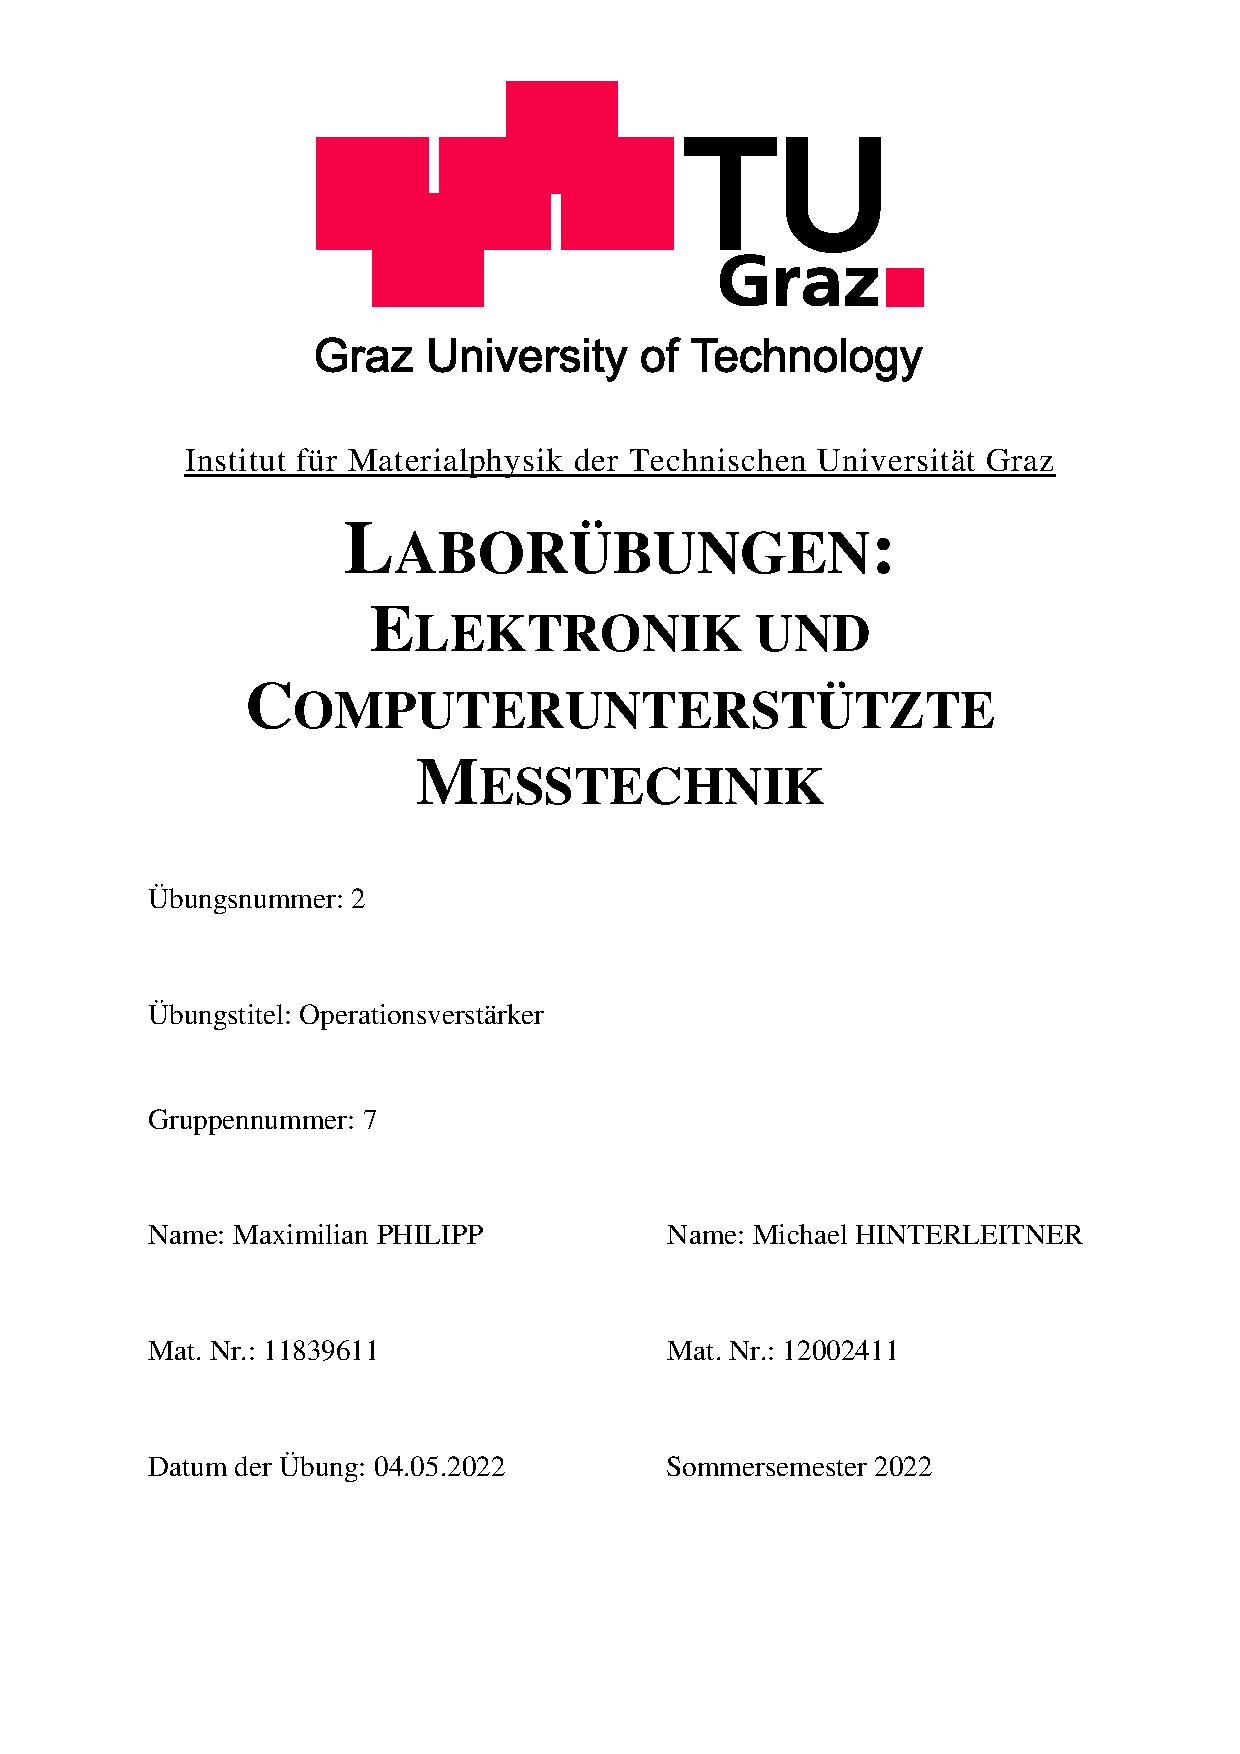
\includepdf{deckblatt2.pdf}
\tableofcontents
\newpage


%\section{Aufgabenstellung}\label{sec:Aufgabenstellung}

% Die nachfolgende Aufgabenstellung wurde von den Laborbetreuern bereitgestellt
% und beinhaltet sowohl Angaben zur Vorbereitung als auch zur praktischen
% Durchführung der Übung:

% zu 1: Aufgabenstellung Das vor der Übung verteilte Aufgabenblatt.
 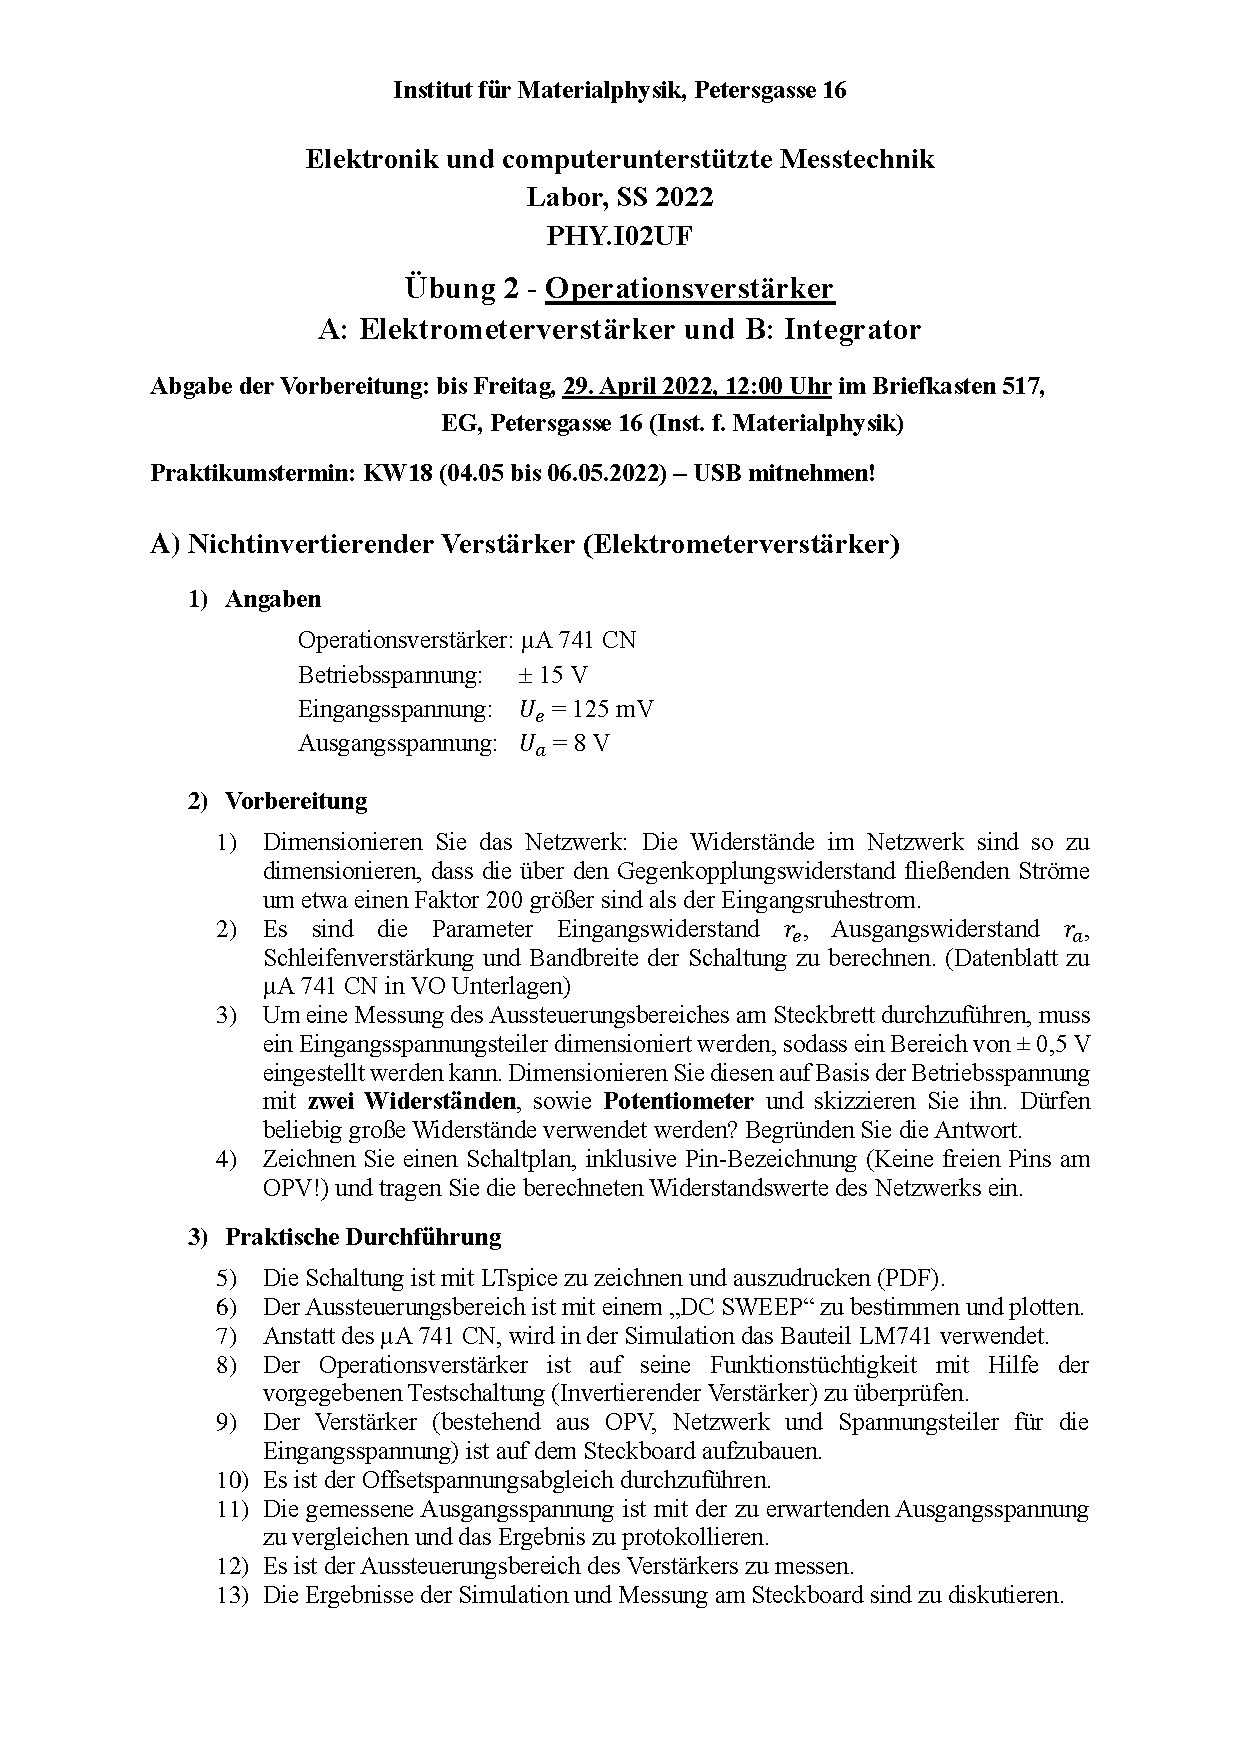
\includepdf[
     pages=-,  % all pages
     addtotoc={
         1, section, 1, Aufgabenstellung, sec:Aufgabenstellung
     }
 ]{angabe.pdf}

% zu 2: Vorbereitung Es sind beide Vorbereitungen dem Protokoll beizufügen.
% \section{Vorbereitung}\label{sec:Vorbereitung}
%Die folgende Vorbereitung wurde vor der Laborübung 
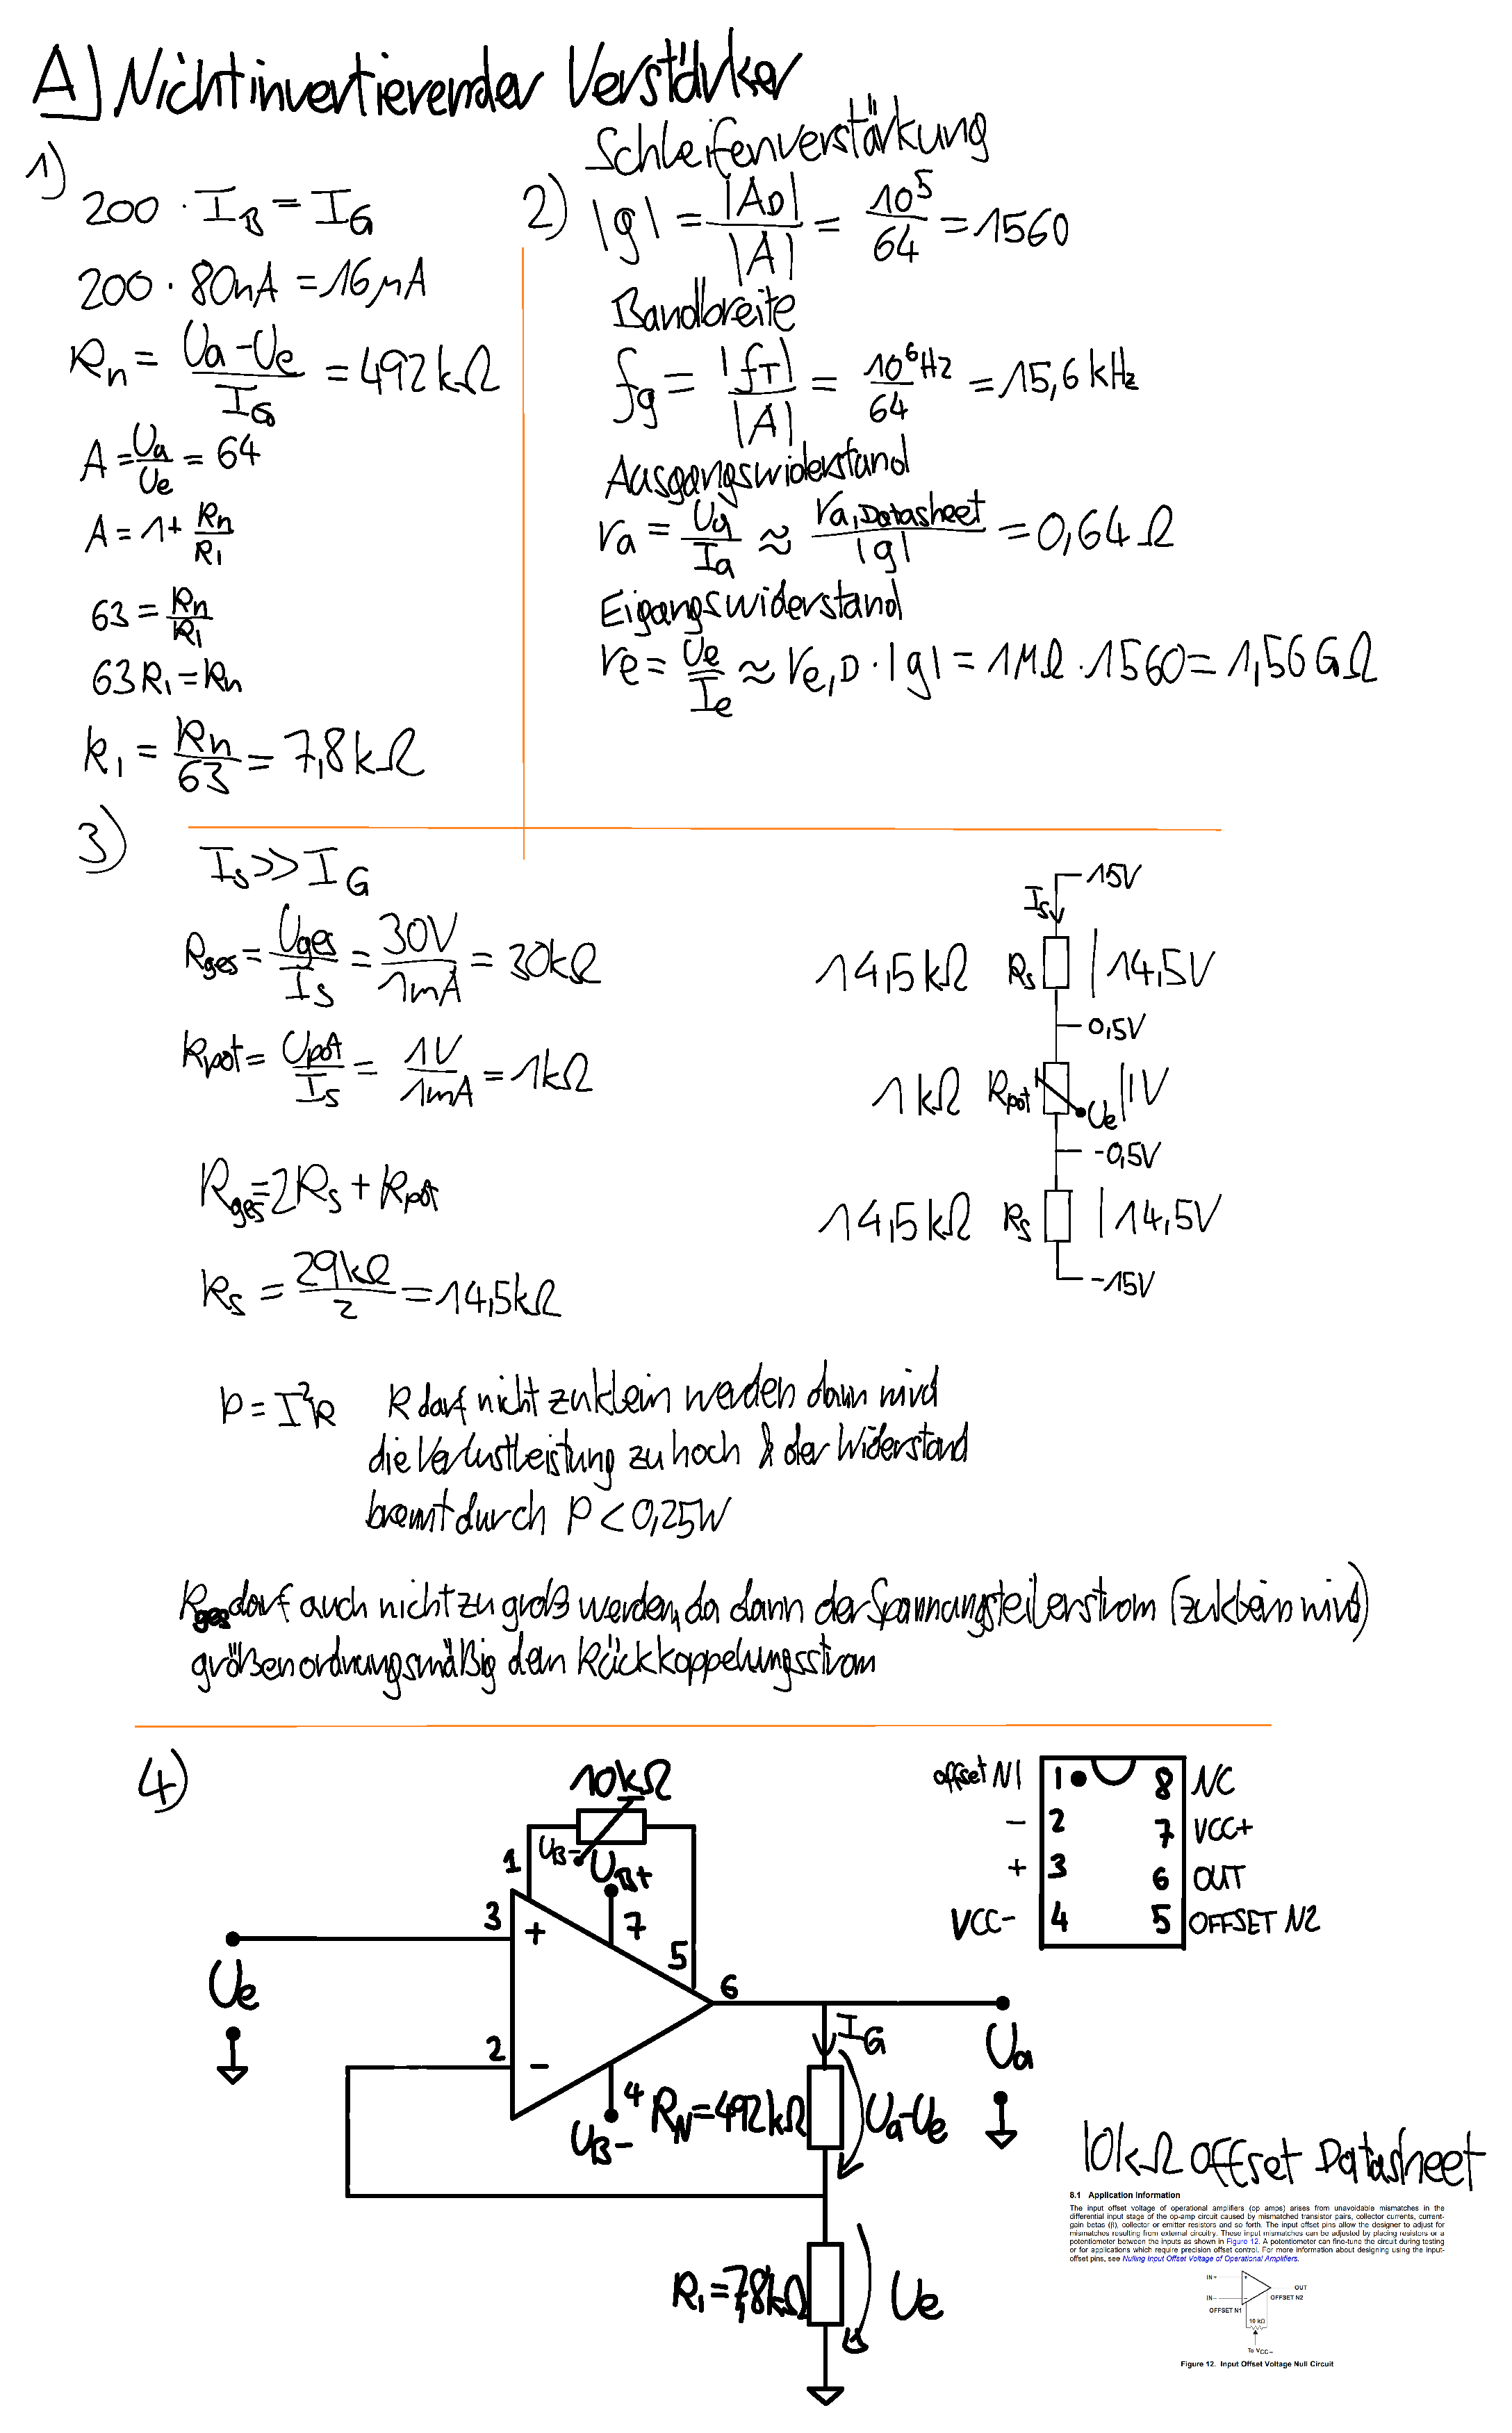
\includepdf[pages=-,
     addtotoc={
         1, section, 2, Vorbereitung, sec:Vorbereitung
     }]{./figures/OpV.pdf}
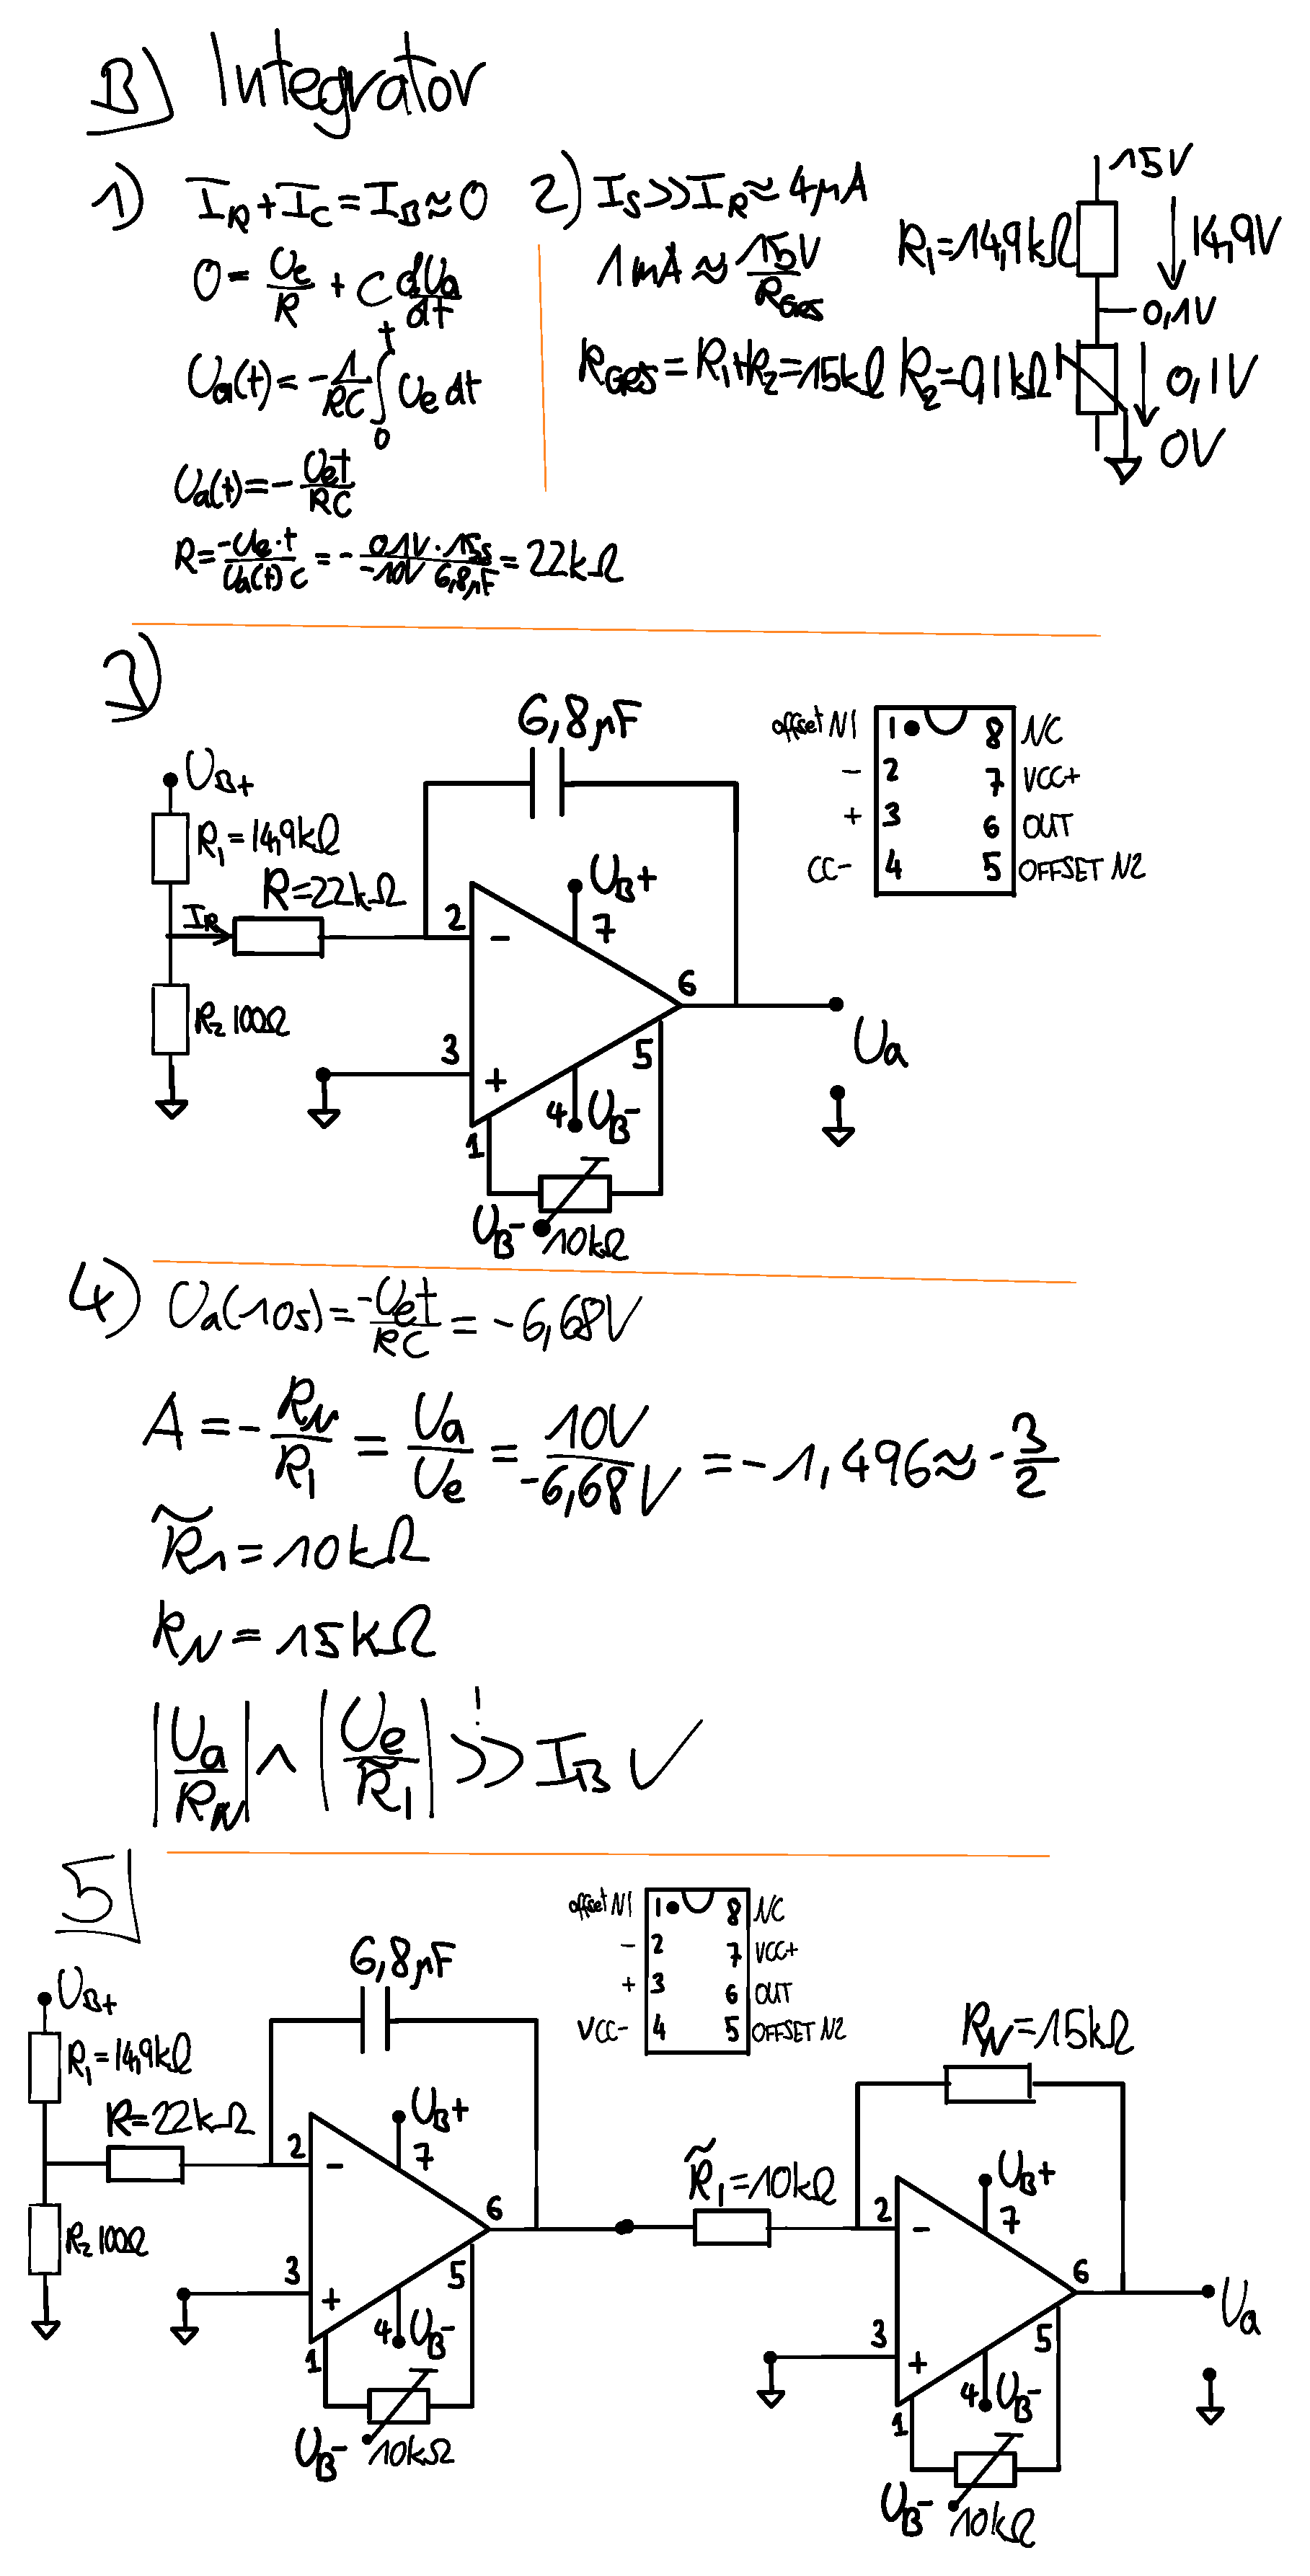
\includepdf[pages=-]{./figures/Integrator1.pdf}
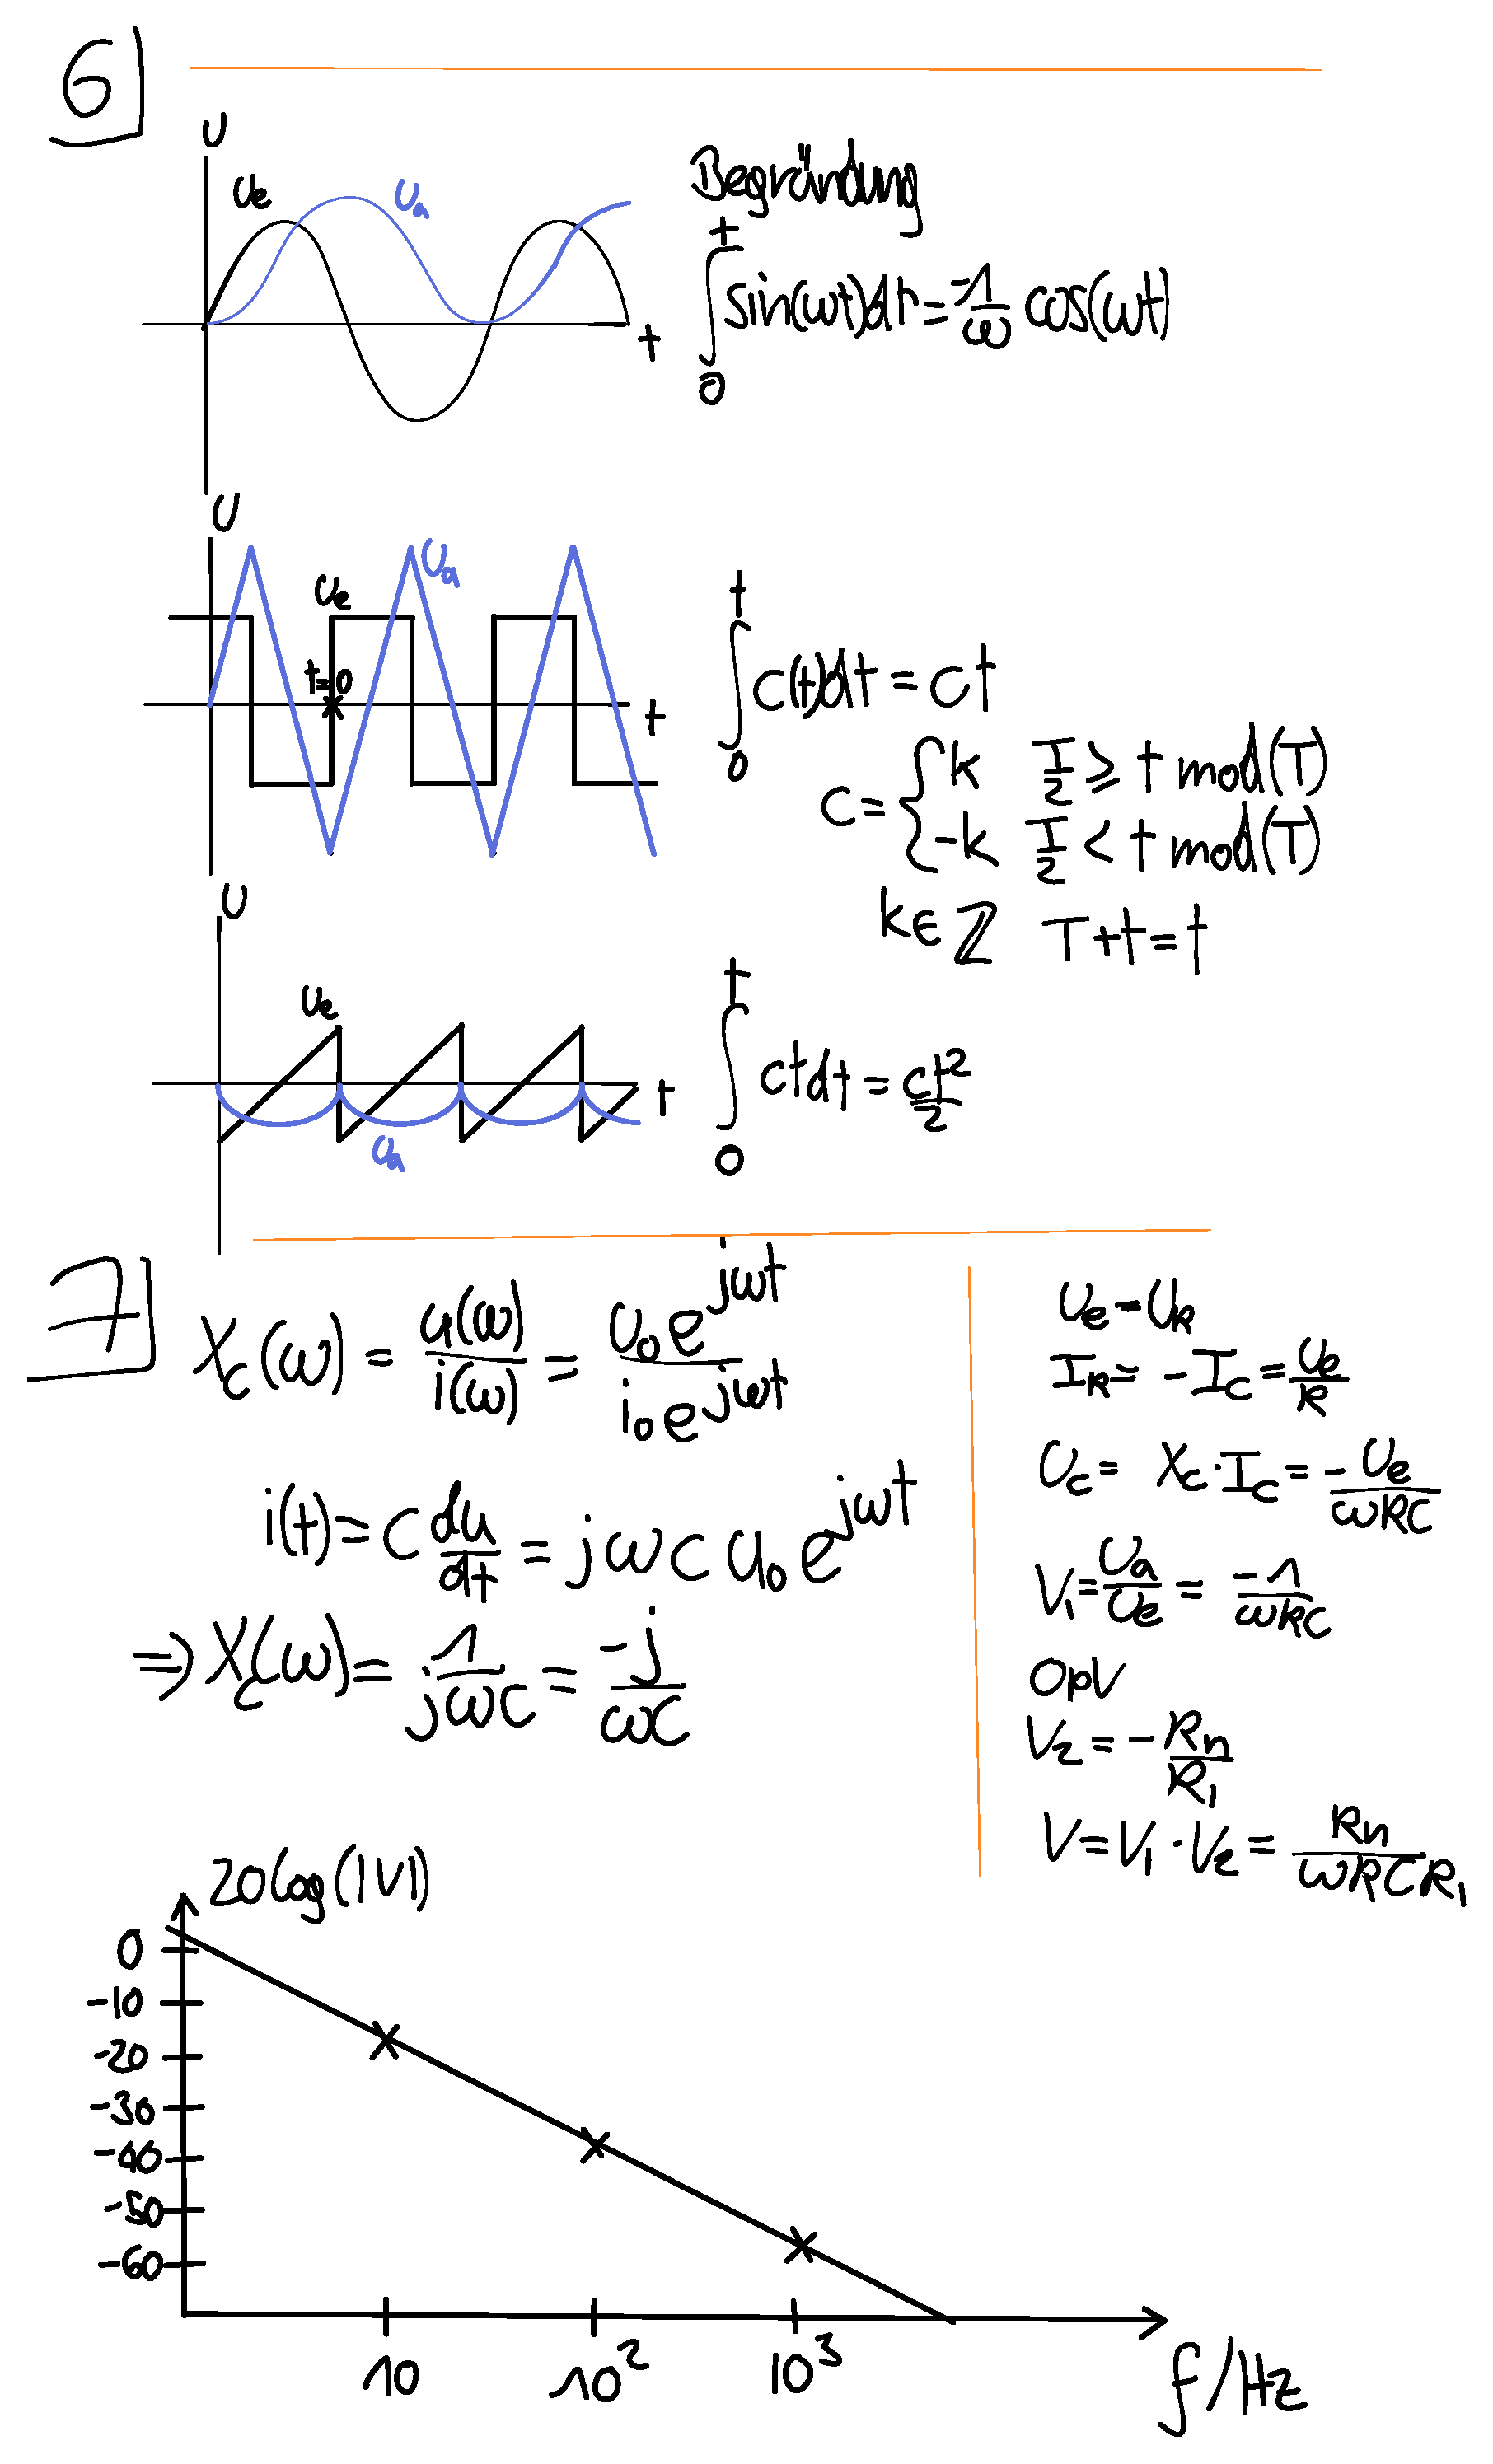
\includepdf[pages=-]{./figures/Integrator2.pdf}
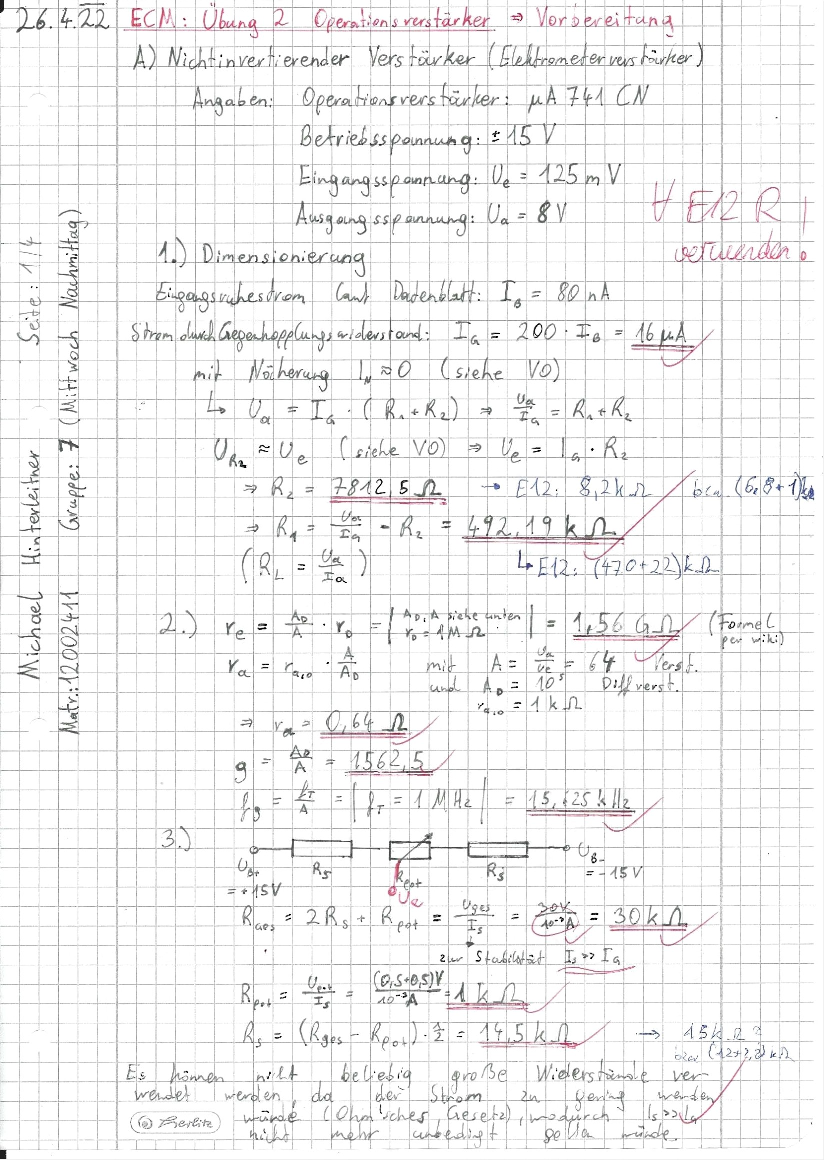
\includepdf[pages=-]{./mh_vorbereitung_opv.pdf}


% zu 3: Grundlagen In den Grundlagen sollen die später verwendeten Formeln
% stehen und kurz erklärt werden, dabei ist es nicht notwendig Formeln
% herzuleiten. Quellenangaben sind an dieser Stelle von Vorteil, weil Sie so
% schnell die betreffenden Stellen in Unterlagen finden. In den Rechnungen
% werden grundlegende Annahmen skizziert und begründet und dann mit diesen
% Annahmen, die für die Schaltungen notwendigen Werte berechnet. Dabei kann
% auch gleich auf die später wirklich verwendeten Werte Bezug genommen werden -
% wir verwenden bei den Widerständen zum Beispiel von den Normwert-Reihen die
% E12 und/oder E24 Serie (nach DIN 41426 bzw. IEC 63).
\section{Grundlagen}\label{sec:Grundlagen}
%in Grundlagen
Operationsverstärker (kurz 'OPV oder 'OpAmp') dienen grundlegend der Verstärkung von 
Gleichspannungen. Sie besitzen einen nicht-invertierenden, der meist mit einem 
Plus, und einen invertierenden Eingang, der mit einem Minus dargestellt wird. Zu 
beachten ist, dass die Verstärkung auf die Differenzspannung der beiden Eingänge 
wirkt. Je zwei zusätzliche Anschlüsse finden sich für die positive und negative 
Betriebsspannung und für den Offsetabgleich, damit bei keiner Eingangsspannung 
auch keine Ausgangsspannung auftritt - dieser wird also in einer externen 
Schaltung durchgeführt.

\begin{figure}[H]
    \centering
    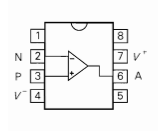
\includegraphics[width=6cm, height=6cm,keepaspectratio]{./figures/pics/pins.PNG}
    \caption{Schematische Darstellung der Pinbelegung eines klassischen Operationsverstärkers. Hierbei bezeichnet 2 den invertierenden, 3 den nicht-invertierenden Eingangskanal, 6 den Ausgang, 4 den Anschluss für die negative sowie 7 den Anschluss für die positive Betriebsspannung, 1 und 5 die Pins für den Offsetabgleich und 8 einen freien Pin.  \cite{tietze}}
    \label{fig:pin_anschl}
\end{figure}

In \autoref{fig:pin_anschl} sind die Pins eines Operationsverstärkers, wie er auch 
in der Laborübung verwendet wurde, zu sehen. Dabei ist zu beachten, dass jeder nicht 
belegte Pin auf Masse gelegt werden soll.

Es gibt vier grundlegende Arten der Verwendung von Operationsverstärkern, darunter
der nicht-invertierende Betrieb, bei dem das Eingangssignal nur auf den nicht-invertierenden 
Kanal gelegt wird und der invertierende auf Masse gelegt wird. Analog funktioniert der invertierende 
Modus, bei dem das Signal anstelle nun an den invertierenden Eingang gelegt wird, wodurch die Ausgangsspannung 
zusätzlich zur Verstärkung noch zum Eingangssignal invertiert wird. Beim Differenzbetrieb werden an 
beide Eingänge Signale angelegt und die Differenzspannung verstärkt. Im Falle des Gleichtaktbetriebs 
liegt das gleiche Eingangssignal an den beiden Eingängen an, wodurch es theoretisch keine Differenzspannung 
und Verstärkung geben sollte - in der Realität resultiert allerdings eine Verstärkung, die als 
Gleichtaktverstärkung bezeichnet wird.

Da der Operationsverstärker ohne zusätzliche Verkopplung sehr stark frequenzabhängig ist und 
nur eine geringe Bandbreite gewünscht verstärkt, wird eine Gegenkopplung vom Ausgang zum Eingang 
durchgeführt, wodurch die Verstärkung zwar abnimmt, die Bandbreite jedoch stark vergrößert wird. 
Die Bandbreite wird wie gewohnt durch die Grenzfrequenz charakterisiert, bei welcher die Verstärkung 
noch \SI{70}{\%} der maximalen beträgt. Wenn nun beispielsweise ein Kondensator in der Rückkopplung verbaut wird, 
handelt es sich um eine Integratorschaltung, die im zweiten Teil der Laborübung untersucht wird.

Die resultierende Verstärkung lässt sich gemäß \autoref{eq:ver} als Verhältnis der Ausgangs- $U_a$ zur Eingangsspannung $U_e$ berechnen.
\begin{equation}
	V=\frac{U_a}{U_e}
	\label{eq:ver}
\end{equation}


% zu 4: Versuchsdurchführung In diesem Punkt wird die Durchführung der
% einzelnen Aufgaben beschrieben. Im Simulationsteil ist die simulierte
% Schaltung mit allen Analyseparametern darzustellen. Im praktischen Teil sind
% die verwendete Geräte sowie die gemessenen Werte der verwendeten Bauteile
% anzugeben. Außerdem sind durchgeführte Funktionsüberprüfungen der Bauteile
% (Dioden, Transistor, etc.) anzuführen. Die Messergebnisse bzw. Oszillogramme
% sind mit Angabe der verwendeten Messgeräte anzugeben. Oszillogramme werden
% vom verwendeten Oszilloskop als Daten auf einen USB-Stick ausgegeben und
% können in das Protokoll aufgenommen werden. Das gleiche gilt für Schaltungen
% bzw. Ergebnissen von Simulationen. Es ist auf eine klare Darstellung der
% Messergebnisse und –auswertung zu achten (Tabellen, geeignete Grafiken). Die
% originalen, während des Versuchs angefertigten Aufzeichnungen sind dem
% Protokoll beizufügen. 
\section{Versuchsdurchführung}\label{sec:versuchsdurchfuehrung}
Für den praktischen Teil an der Steckplatine wurden Widerstände der E12-Reihe,
mit denen die in der Vorbereitung angegebenen respektive errechneten Werte
angenähert wurden, verwendet. 

Die verwendeten Geräte sind \autoref{tab:geraeteliste} zu entnehmen.

\begin{table}
  \caption{Tabelle der verwendeten Geräte}
  \label{tab:geraeteliste}
  \centering
  \begin{tabular}{l|l}
    \hline
   \multicolumn{2}{ c }{\textbf{Geräteliste}} \\
    \hline
    \textbf{Gerät/Bauelement} & \textbf{Typ} \\
    \hline
    Oszilloskop & \textit{Tektronix TDS 2002}\cite{oszilloscope}\\
    Funktionsgenerator & \textit{H-TRONIC FG250D}\cite{funktionsgenerator} \\
    Netzgerät & nicht bestimmbar\\
    Multimeter & \textit{Fluke 175 TrueRMS}\cite{fluke175} \\
    OPV & \textit{$\mu$A741}\\
    \hline
  \end{tabular}
\end{table}

\subsection{Elektrometerverstärker}

% 5) Die Schaltung ist mit LTspice zu zeichnen und auszudrucken (PDF).
\subsubsection{Simulation} \label{sec:Versuchsim}

% TODO text
Zur Simulation des Elektrometerverstärkers wird das Programm
\textit{LTSPICE} verwendet. Der Aufbau erfolgt analog zum skizzierten
Schaltplan in \autoref{fig:sim_elektrometer_schaltung}. Hier wurde das gleiche
Bauteil wie im Kapitel \nameref{sec:Aufgabenstellung} verwendet, nämlich der $\mu$A741.

\begin{figure}[H]
  \centering
  % TODO LTSPICE aufbau der Elektrometer
    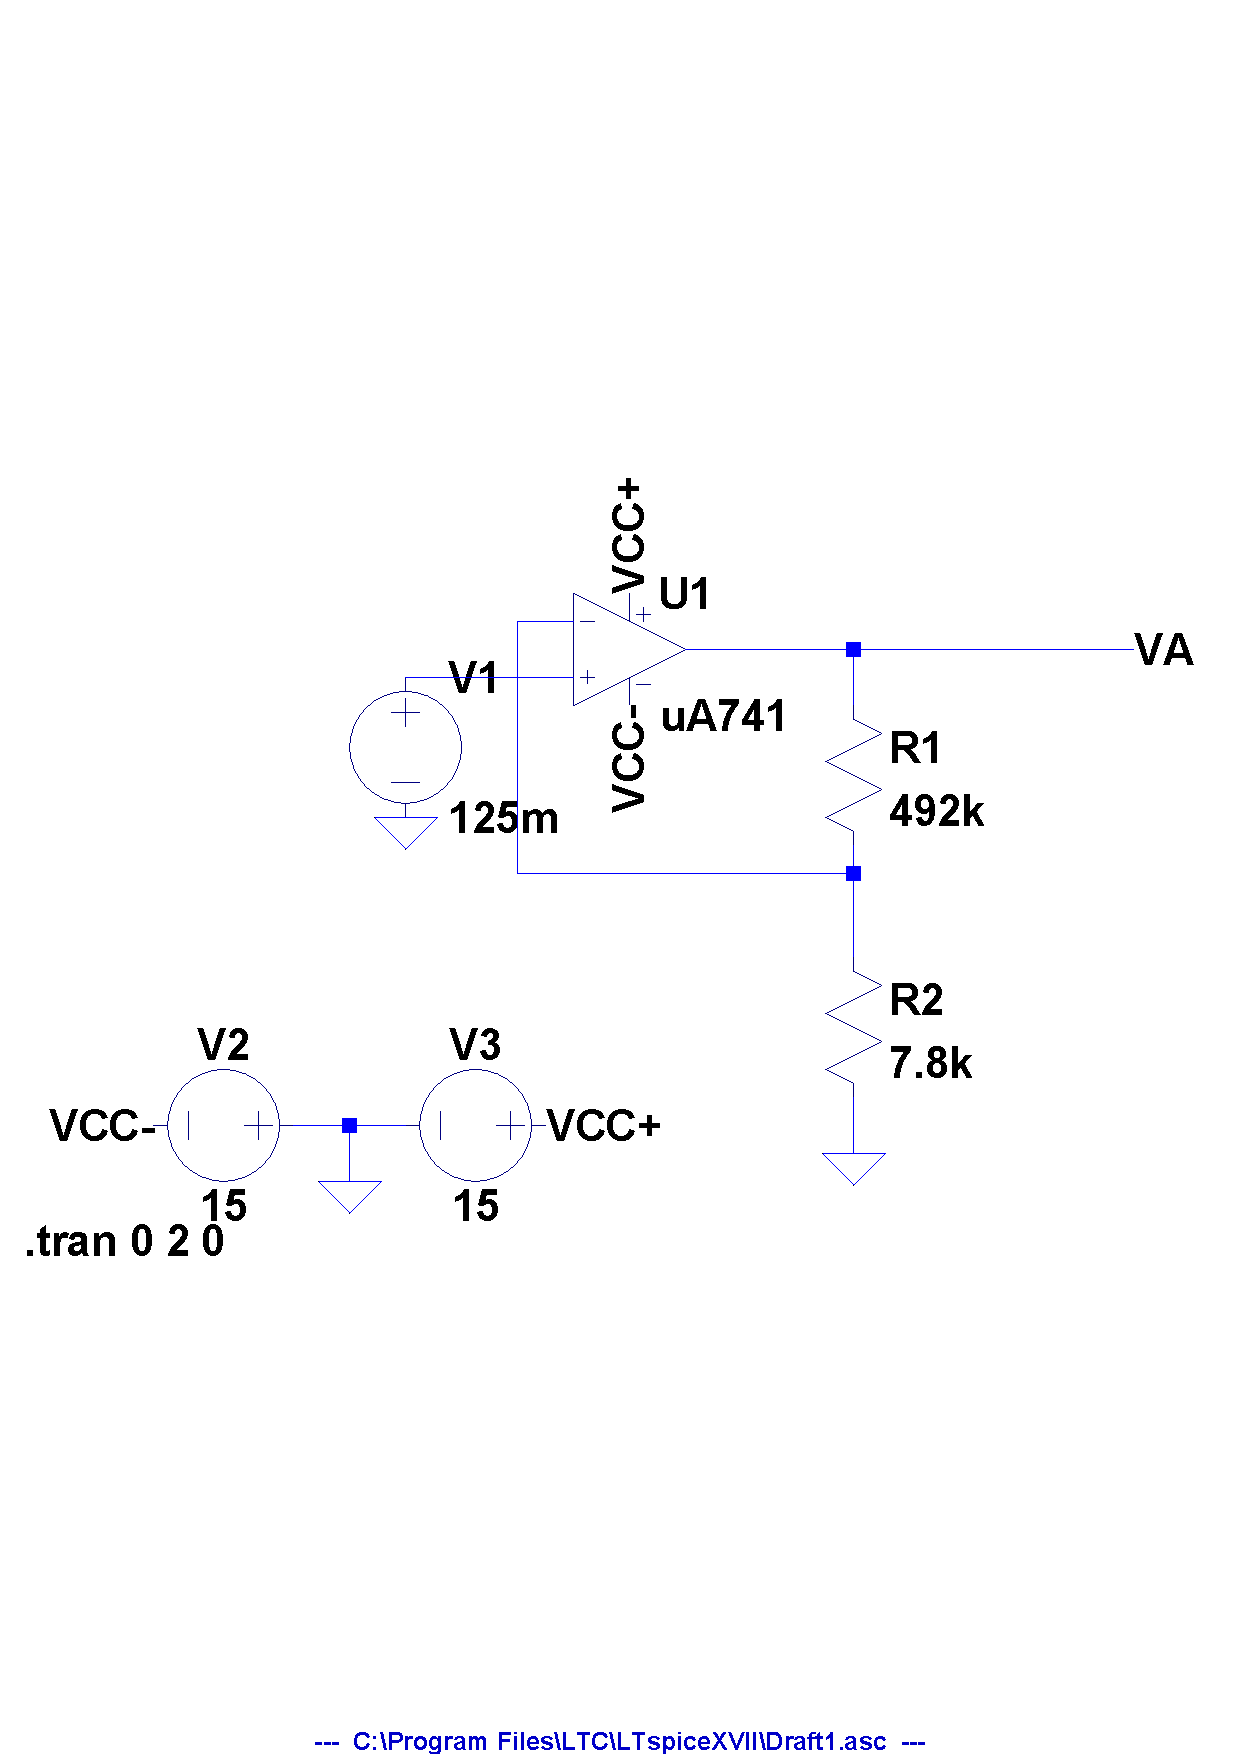
\includegraphics[width=0.95\textwidth]{./figures/elektrometer/sim/sim_schaltung.pdf}
  \caption{Dies ist die Elektrometerverstärkerschaltung; aufgebaut in \textit{LTSPICE}.}
  \label{fig:sim_elektrometer_schaltung}
\end{figure}


% 6) Der Aussteuerungsbereich ist mit einem „DC SWEEP“ zu bestimmen und plotten.
% 7) Anstatt des µA 741 CN, wird in der Simulation das Bauteil LM741 verwendet.
% NEIN fehler in der Angabe sollte UA741 bauteil sein
\paragraph{Untersuchung des Aussteuerungsbereichs} \label{sec:mess_aussteuerungsbereich}

Um den Aussteuerungsbereich zu bestimmen, wurde ein DC-Sweep der
Eingangsspannung durchgeführt und die Ausgangsspannung in Abhängigkeit der
Eingangsspannung graphisch, wie in \autoref{fig:sim_elektrometer_dcsweep}
ersichtlich, dargestellt. Es musste in der Simulation kein
Offsetspannungsabgleich durchgeführt werden.

\begin{figure}[H]
  \centering
  % TODO LTSPICE dc sweep von ausgangsspannung 
    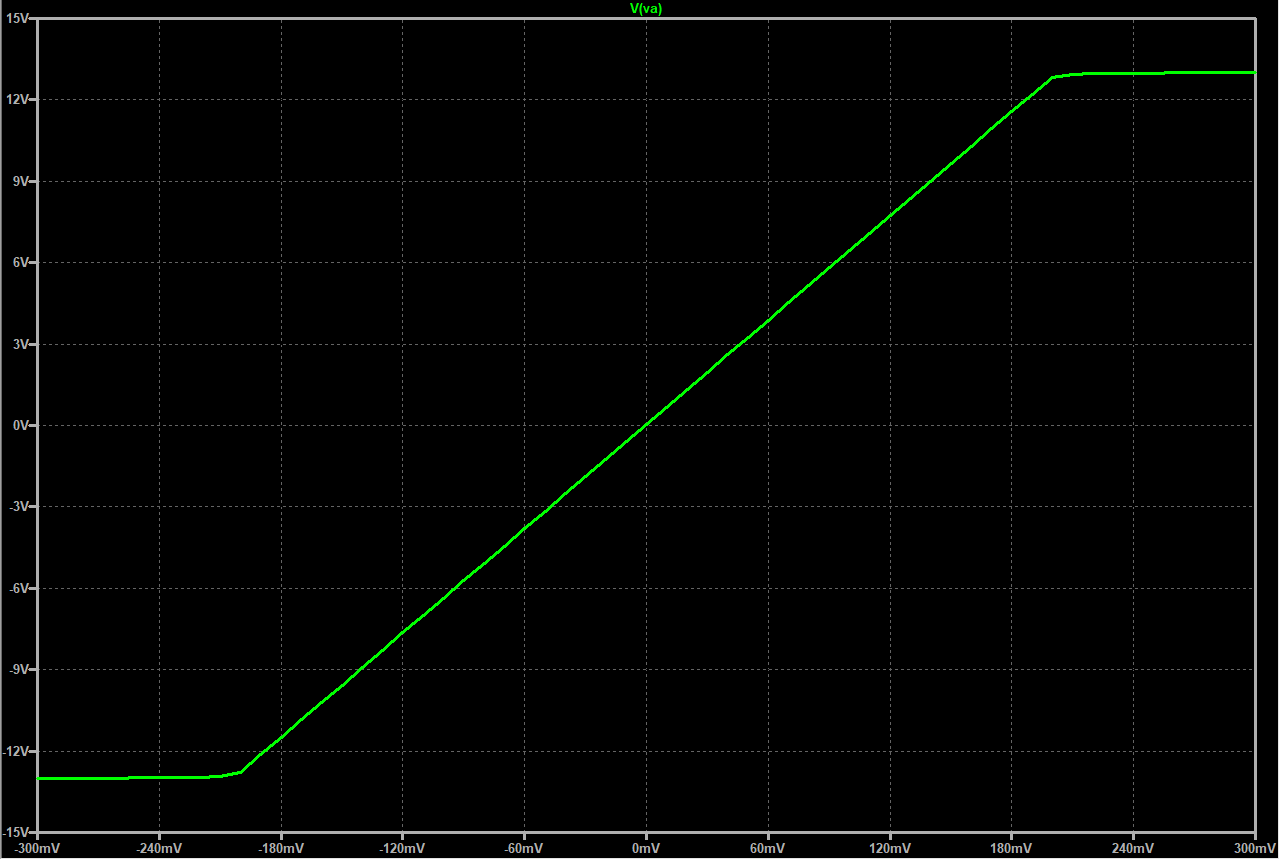
\includegraphics[width=0.95\textwidth]{./figures/elektrometer/sim/aus_sweep.png}
  % TODO check spice directive
  \caption{Die Schaltung aus \autoref{fig:sim_elektrometer_schaltung} wurde auf
    den Aussteuerungsbereich untersucht, indem ein DC-Sweep durchgeführt wurde.
    Hier ist die Ausgangsspannung $VA$ über die Eingangsspannug $V1$
    aufgetragen. Die SPICE-Directive der Simulation ist \texttt{.dc V1 -0.3 0.3 0.01}}
  \label{fig:sim_elektrometer_dcsweep}
\end{figure}

\subsubsection{Steckbrett} \label{sec:elektrometer_steckbrett}
Bevor die Schaltung zunächst aufgebaut werden kann muss die
Funktionstüchtigkeit des OPVs getestet werden, damit keine unzuverlässigen
Komponentten verwendet werden. Daraufhin wird eine Impedanzwandlerschaltung mit
dem funktionstüchtigen OPV gebaut, mit welcher leicht der
Offsetspannungsabgleich gemacht werden kann.


\paragraph{Testschaltung}
% 8) Der Operationsverstärker ist auf seine Funktionstüchtigkeit mit Hilfe der
% vorgegebenen Testschaltung (Invertierender Verstärker) zu überprüfen.
Zur Untersuchung der Funktionstüchtigkeit des OPVs wurde die im Labor vorhandene
Testschaltung, siehe \autoref{fig:testschaltung}, verwendet. 

\begin{figure}[H]
  \centering
  % TODO grafik einfuegen
    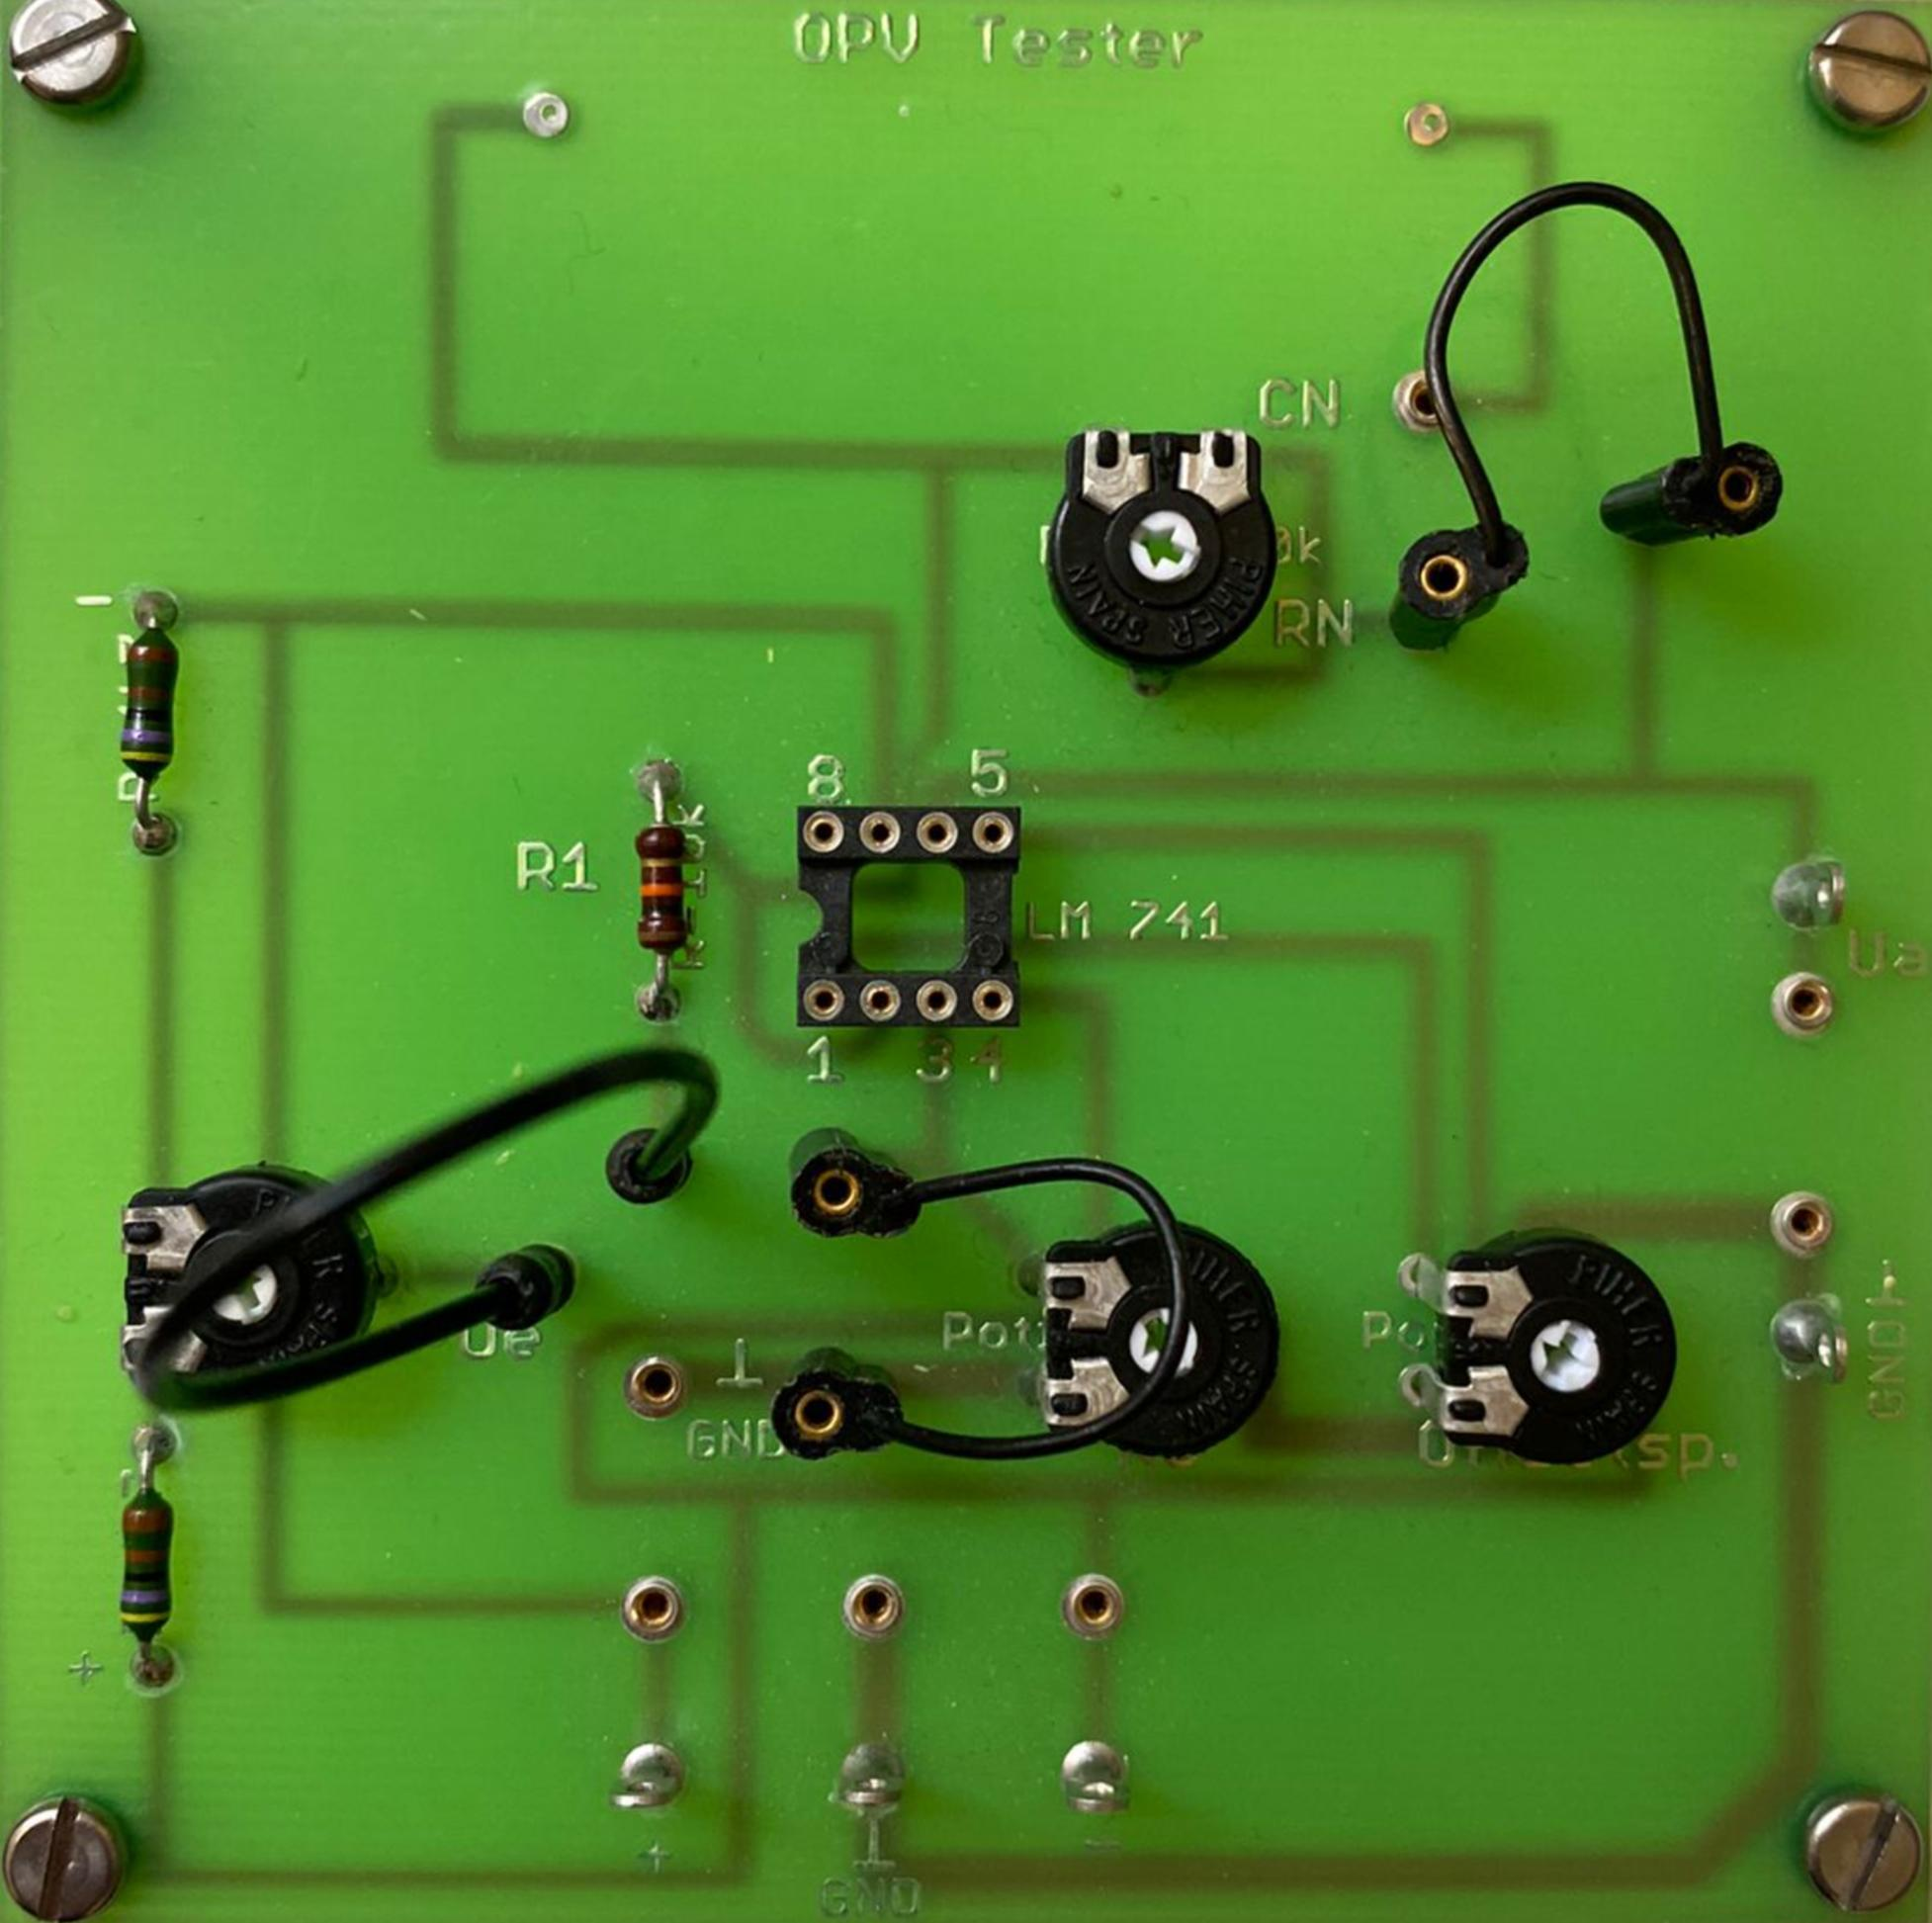
\includegraphics[width=0.95\textwidth]{./figures/testschaltung.jpeg}
  \caption{Die vorhandene Testschaltung als invertierender Verstärker.}
  \label{fig:testschaltung}
\end{figure}

Diese Schaltung wurde verwendet, um zu überprüfen, ob der OPV noch immer die
gewünschten Eigenschaften für positive und negative Verstärkungen aufweist. Dies
wurde durch Variieren des Potentiometers (und somit Variieren der
Eingangsspannung) und dem Messen der Ausgangsspannung erfolgreich überprüft.

% 9) Der Verstärker (bestehend aus OPV, Netzwerk und Spannungsteiler für die
% Eingangsspannung) ist auf dem Steckboard aufzubauen.
\paragraph{Aufbau}
Im Gegensatz zu der in \autoref{fig:sim_elektrometer_schaltung} ersichtlichen
Schaltung wird am Steckbrett ein Spannungsteiler als \SI{100}{mV}
Spannungsquelle verwendet. Dazu wurden ein \SI{15.0}{\kilo\ohm} und ein
\SI{14.96}{\kilo\ohm} mit einem \SI{1}{\kilo\ohm} Poti verwendet um eine wie in
der \autoref{sec:Vorbereitung} ersichtlichen Spannungsteiler zu bauen. Welcher
an der Betriebsspannung $VCC$ \SI{+15}{\volt} und der negativen
Betriebsspannung $VCC-$ \SI{-15}{\volt} anliegt, um eine, durch das dritte
mittelere Bein des Poti abgreifbare, Spannung $V1$ zu erzeugen, welche
mindestens einen, durch das Poti einstellbaren, Bereich von
\SIrange{-500}{500}{\milli\volt} abdecken kann. Weiters wurden die in der
\autoref{fig:sim_elektrometer_schaltung} ersichtlichen Widerstände
\SI{492}{\kilo\ohm} und \SI{7.8}{\kilo\ohm} durch folgende E12-Reihe
Wiederstände \SI{470}{\kilo\ohm} mit \SI{22}{\kilo\ohm} und \SI{6.8}{\kilo\ohm}
mit einem \SI{1}{\kilo\ohm} Poti, welcher verwendet werden kann um die
Ungenauigkeiten der E12 Widerstände beim Verstärkungsfaktor ausbessern zu
können.

\begin{figure}[H]
  \centering
  % TODO Beschriftung der Grafik 
    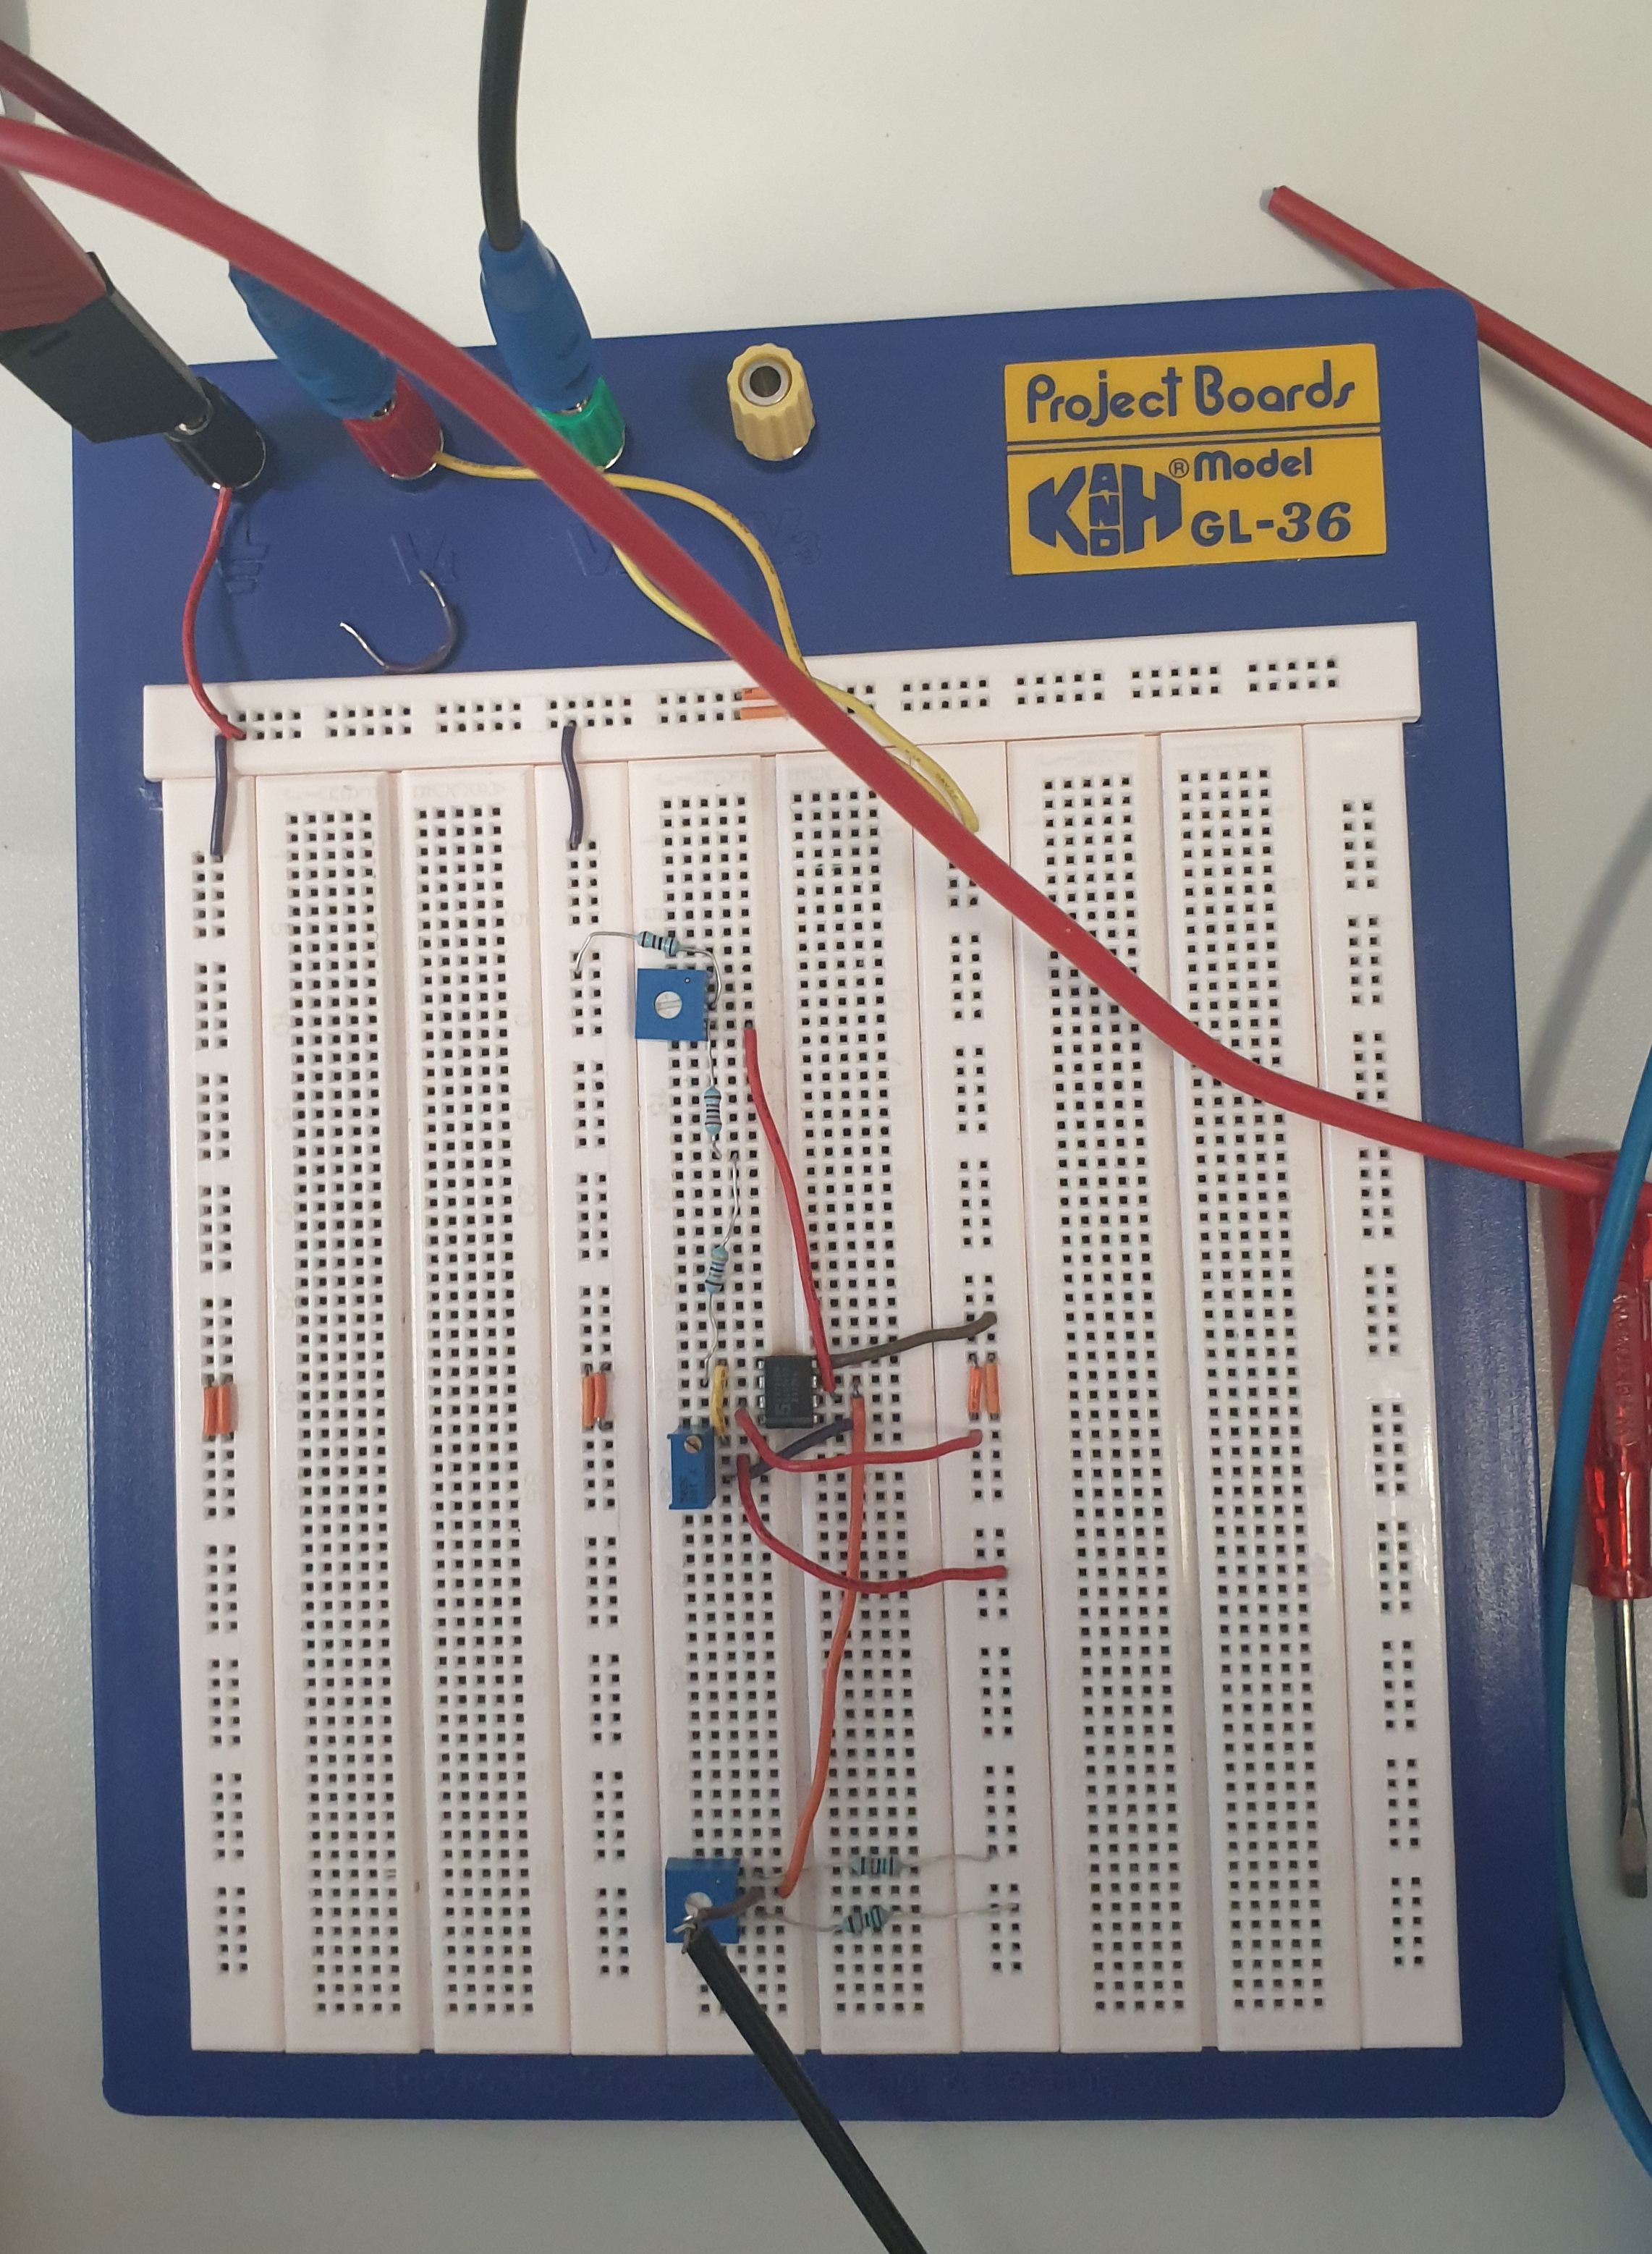
\includegraphics[width=0.95\textwidth]{./figures/elektrometer/steckbrett.png}
  \caption{Der Aufbau des Elektrometerverstärkers am Steckbrett der Schaltung von
  \autoref{fig:sim_elektrometer_schaltung}}
  \label{fig:ver_elektromete_aufbau}
\end{figure}

% 10) Es ist der Offsetspannungsabgleich durchzuführen.
\paragraph{Offsetabgleich}\label{sec:offsetabgleich}
Um den Offsetsspannungableich durchführen zu können, ist zuerst mal ein
Impedanzwandler aufgebaut worden, wodurch das Abgleichen sich zum Abstimmen
der Eingangsspannug zur Ausgangsspannung vereinfachte. Dies wurde durch ein
extern beschaltetes Potentiometer bewerkstelligt, welches die Rolle eines
Spannungteilers spielte. Der Offsetabgleich wurde bei einer Spannung von
\SI{125.4}{\milli\volt} gemacht.

% 11) Die gemessene Ausgangsspannung ist mit der zu erwartenden Ausgangsspannung
% zu vergleichen und das Ergebnis zu protokollieren.
\paragraph{Beschaltung als Elektrometerverstärker}
Nun wurde die Rückkopplung durch einen Spannungsteiler, wie in
\autoref{fig:sim_elektrometer_schaltung} ersichtlich, statt dem Kurzschluss vom
Ausgang zum invertierenden Eingang eingebaut. Zunächst gab es Probleme mit dem
Aufnehmen der Verstärkung, da der Ground einen Wackelkontakt bekommen hat,
welcher durch leichtes drehen des Anschlusses repariert werden konnte.
Nun konnte die $U_a$ und $U_e$ des Elektrometerverstärker gemessen werden. Dies
wurde mittels zwei Multimeter \cite{fluke175} bewerkstelligt, indem wie in
\autoref{fig:sim_elektrometer_schaltung} ersichtlich über die Spannungsquelle
$V1$ und von $VA$ zu Masse gemessen wurde.

Der Poti im Spannungsteiler erlaubte und die Verstärkung genau einzustellen
jedoch war eine genauere Einstellungen schwer per Hand möglich digital
ansteuerbares poti wäre nice.

\begin{equation}
  U_a = \SI{8.03}{\volt} \quad @\, U_e = \SI{125.0}{\milli\volt}
  \label{eq:messwert_elektro_ausgang_eingang}
\end{equation}

% 12) Es ist der Aussteuerungsbereich des Verstärkers zu messen.
\paragraph{Untersuchung des Aussteuerungsbereichs} \label{sec:Versuchohnekond}
Um den Aussteuerungsbereich untersuchen zu können wurde der
Eingangsspannugsteiler so dimensioniert, dass dieser an die Grenzen der
Verstärkung des OPVs bis zu der Betriebsspannung treiben kann. Da die
Eingangsspannug von \SIrange{-500}{500}{\milli\volt} und der Verstärkungsfaktor
circa \num{64} beträgt ist es leicht bis über die Betriebsspannung hinaus zu
verstärken.

%TODO hier fucker

\begin{table}[H]
  \caption{Gemessene Ausgangs- und Eingangspannungen der Elektrometerschaltung
  zur Untersuchung des Aussteuerungsbereichs\\
  $U_a \dots$ Ausgangsspannung \\
  $U_e \dots$ Eingangspannung \\
  }
  \label{tab:mess_elektro_aussteurerung}
  \centering
  \begin{tabular}{lrrrrrr}
	\toprule
	{} & $P_1$ / \si{\watt} & $U$ / \si{\volt} & $U_1$ / \si{\volt} & $I_1$ / \si{\ampere} & $U_2$ / \si{\volt} \\
	\midrule
	0  & 7.4                & 160.0            & 161.0              & 0.200                & 14.4               \\
	\bottomrule
\end{tabular}

\end{table}


% 13) Die Ergebnisse der Simulation und Messung am Steckboard sind zu diskutieren.

\subsection{Integrator}
% 1) Der Umkehrintegrator ist mit LTspice zu zeichnen und als Abbildung zu speichern.

\subsubsection{Simulation}
Zur Simulation der Integratorschaltung wird das Programm
\textit{LTSPICE} verwendet. Der Aufbau erfolgt analog zum skizzierten
Schaltplan in \autoref{fig:sim_integrator_schaltung}. 

\begin{figure}[H]
  \centering
  % TODO LTSPICE aufbau der Elektrometer
    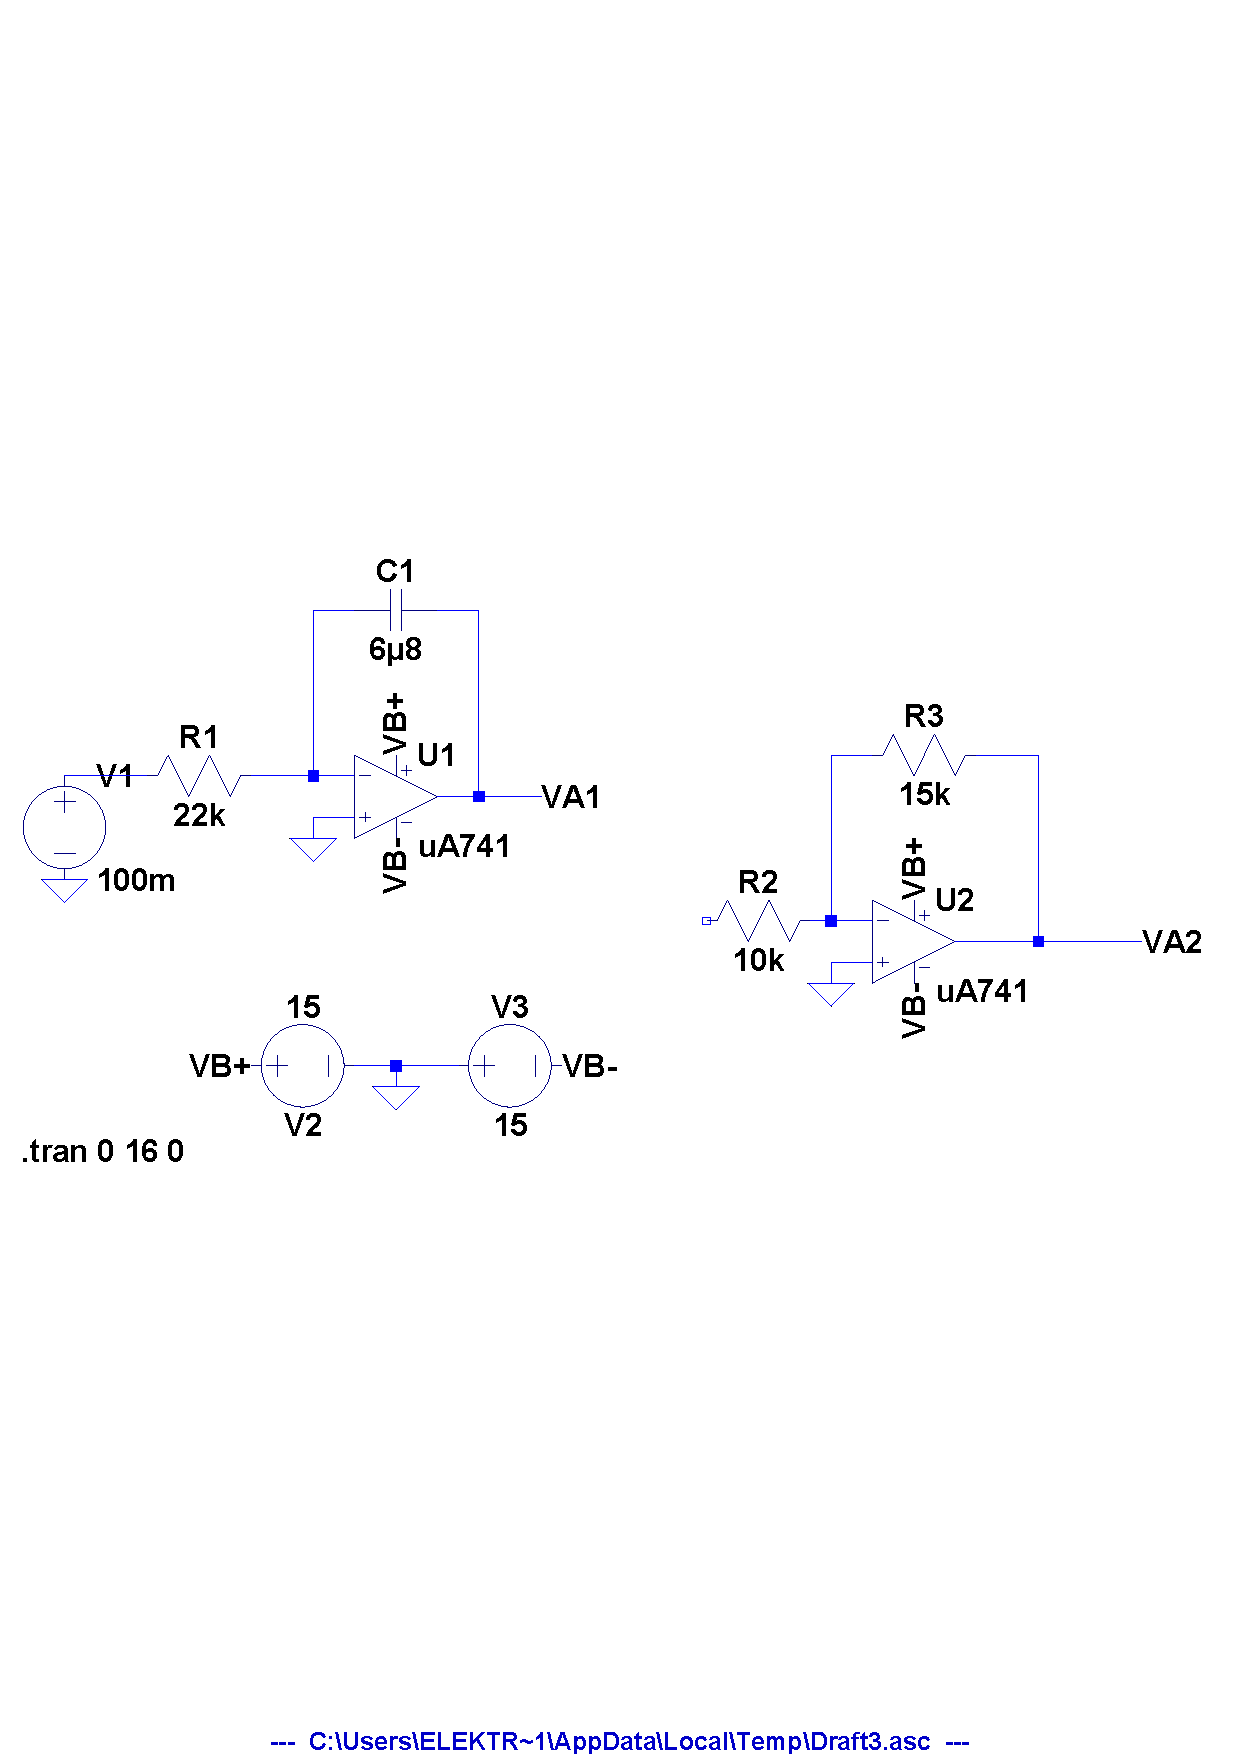
\includegraphics[width=0.95\textwidth]{./figures/integrator/sim/umkehr_int/schalt_umkehr_100mv.pdf}
  \caption{Dies ist die Integratorschaltung aufgebaut in \textit{LTSPICE}}
  \label{fig:sim_integrator_schaltung}
\end{figure}

% 2) Die Integrationsdauer der Schaltung ist mit einer konstanten Spannungsquelle zu
% simulieren. Die Ergebnisse sind mit der Vorbereitung zu vergleichen.
\paragraph{Integrationszeit}
Um die Integrationszeit, die bei \SI{-10}{\volt} erreicht wird, zu bestimmen, wurde eine zeitliche 
Transienten-Analyse durchgeführt, wobei eine konstante Spannungsquelle von \SI{100}{\milli\volt} verwendet
wurde. In \autoref{fig:sim_integrator_integrationszeit} ist die auftretende Ausgangsspannung in
Abhängigkeit der Zeit zu sehen.

% TODO text

\begin{figure}[H]
  \centering
  % TODO LTSPICE trans anal von lade vorgang 
    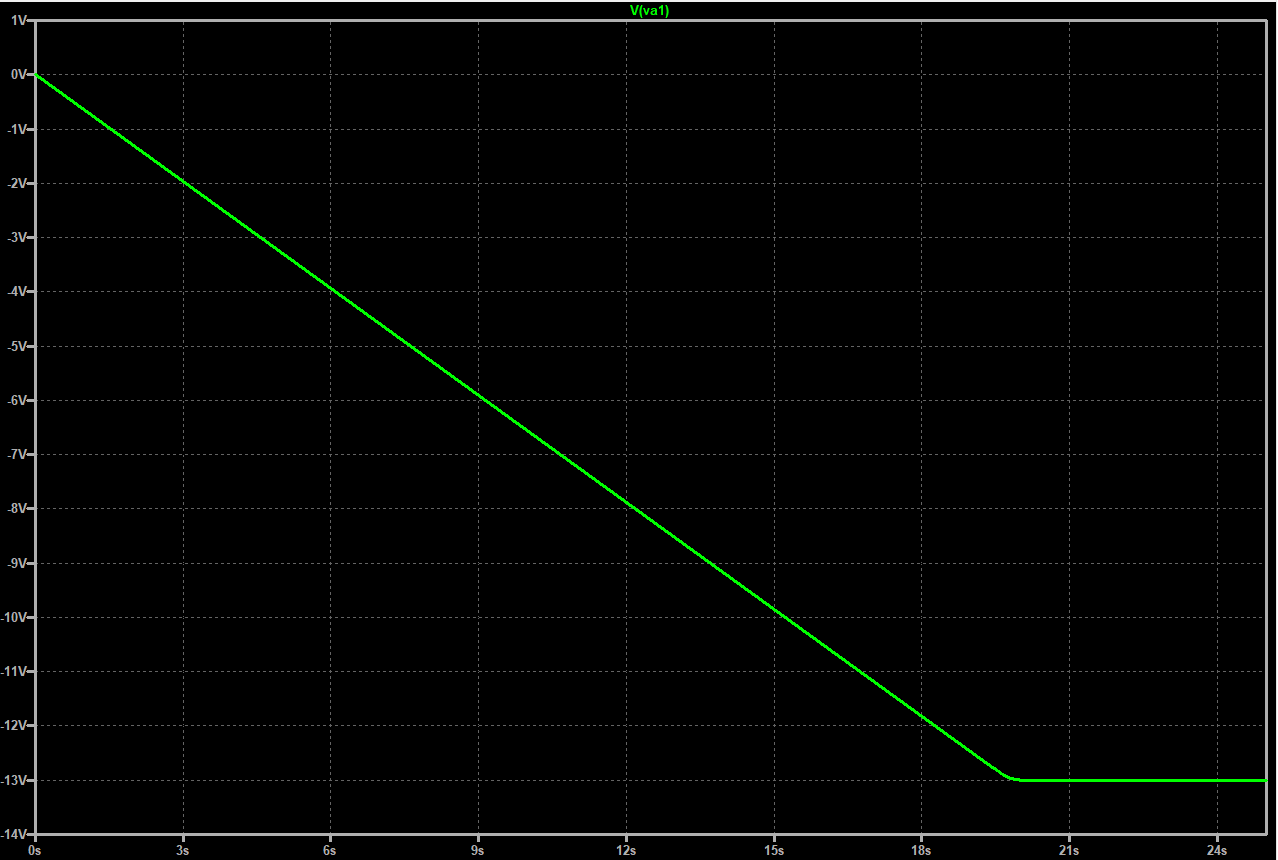
\includegraphics[width=0.95\textwidth]{./figures/integrator/sim/umkehr_int/dauer_aussteu.png}
  % TODO check spice directive
  \caption{Die Schaltung aus \autoref{fig:sim_integrator_schaltung} wurde auf
  die Integrationszeit untersucht in dem eine Transiente-Analyse vom
  Ladevorgang gemacht wurde. Die Simulation SPICE-Directive ist \texttt{.tran 0 25 0} 
  bei einer Eingangspannung $V1$ von \SI{100}{\milli\volt}.}
  \label{fig:sim_integrator_integrationszeit}
\end{figure}

\subsubsection{Steckbrett}
% 3) Der OPV ist auf die Funktionstüchtigkeit zu prüfen. (siehe Aufgabe A, Punkt 8)
% 5) Es ist der Offsetspannungsabgleich durchzuführen.
Wie in \autoref{sec:offsetabgleich} erklärt, wurde nochmals mit der
Impdanzwandlerschaltung die Funktionstüchtigkeit überprüft. Ebenfalls wurde
gleich die Offsetabgleich nochmals überprüft. Jedoch musste dieser nicht
angepasst werden, da noch immer alles kalibriert war.

% 4) Der Umkehrintegrator (bestehend aus OPV, Netzwerk und Spannungsteiler) ist auf
% dem Steckboard aufzubauen.
% 6) Die aufgebaute Schaltung ist in Betrieb zu nehmen und die Integrationszeit zu
% protokollieren (Stoppuhr). Die Messung ist fünfmal zu wiederholen.
\paragraph{Integrationszeit}
Nun wurde die charakteristische Ingetrationszeit der Schaltung bestimmt. Indem
zuerst der Kondensator, bis das Multimeter am Ausgang \SI{0}{\mV} anzeigte,
entladen wurde und danach ist die Zeit des Ladens, die die Schaltung brauchte
um die geforderte Spannung von \SI{10}{\volt} am Ausgang zu haben, gemessen.
Dies wurde 6 mal wiederholt um eine Mittelung der Messergebnisse durchführen zu
können.

\begin{table}
  \caption{Messungen der Integrationszeit der realen Integratorschaltung aus
  \autoref{fig:sim_integrator_schaltung}, wobei $T$ die Ladezeit bis am Ausgang
  \SI{10}{\volt} anliegt. Bei einem Ladespannung \SI{91.8}{\milli\volt}, einem
  Widerstand von \SI{21.9}{\kilo\ohm} und einer Kapazität von
  \SI{6.8}{\micro\farad} }
  \label{tab:messungen_integration}
  \centering
  \begin{tabular}[c]{S}
    {$T$ / \si{\second}} \\
    17.20 \\
    16.42 \\
    16.90 \\
    16.89 \\
    17.32 \\
    17.21 \\
  \end{tabular}
\end{table}


% 7) Die Schaltung (und Simulation) ist mit verschiedenen Spannungsquellen (Sinus,
% Rechteck, Dreieck) zu testen. Protokollieren und vergleichen Sie die Ergebnisse.
% Nutzen Sie dazu Oszilloskop und Frequenzgenerator.
\paragraph{Untersuchung Verschiedene Eingangssignale}
Nun wurde die Integrationsfähigkeit der Schaltung durch Einspeisen
verschiedener Eingangssignal qualitative untersucht. Dazu wurde zunächst ein
Sinuseingangssignal, siehe \autoref{fig:mess_integrator_sinussignal}, verwendet.
 
\begin{figure}[H]
  \centering
    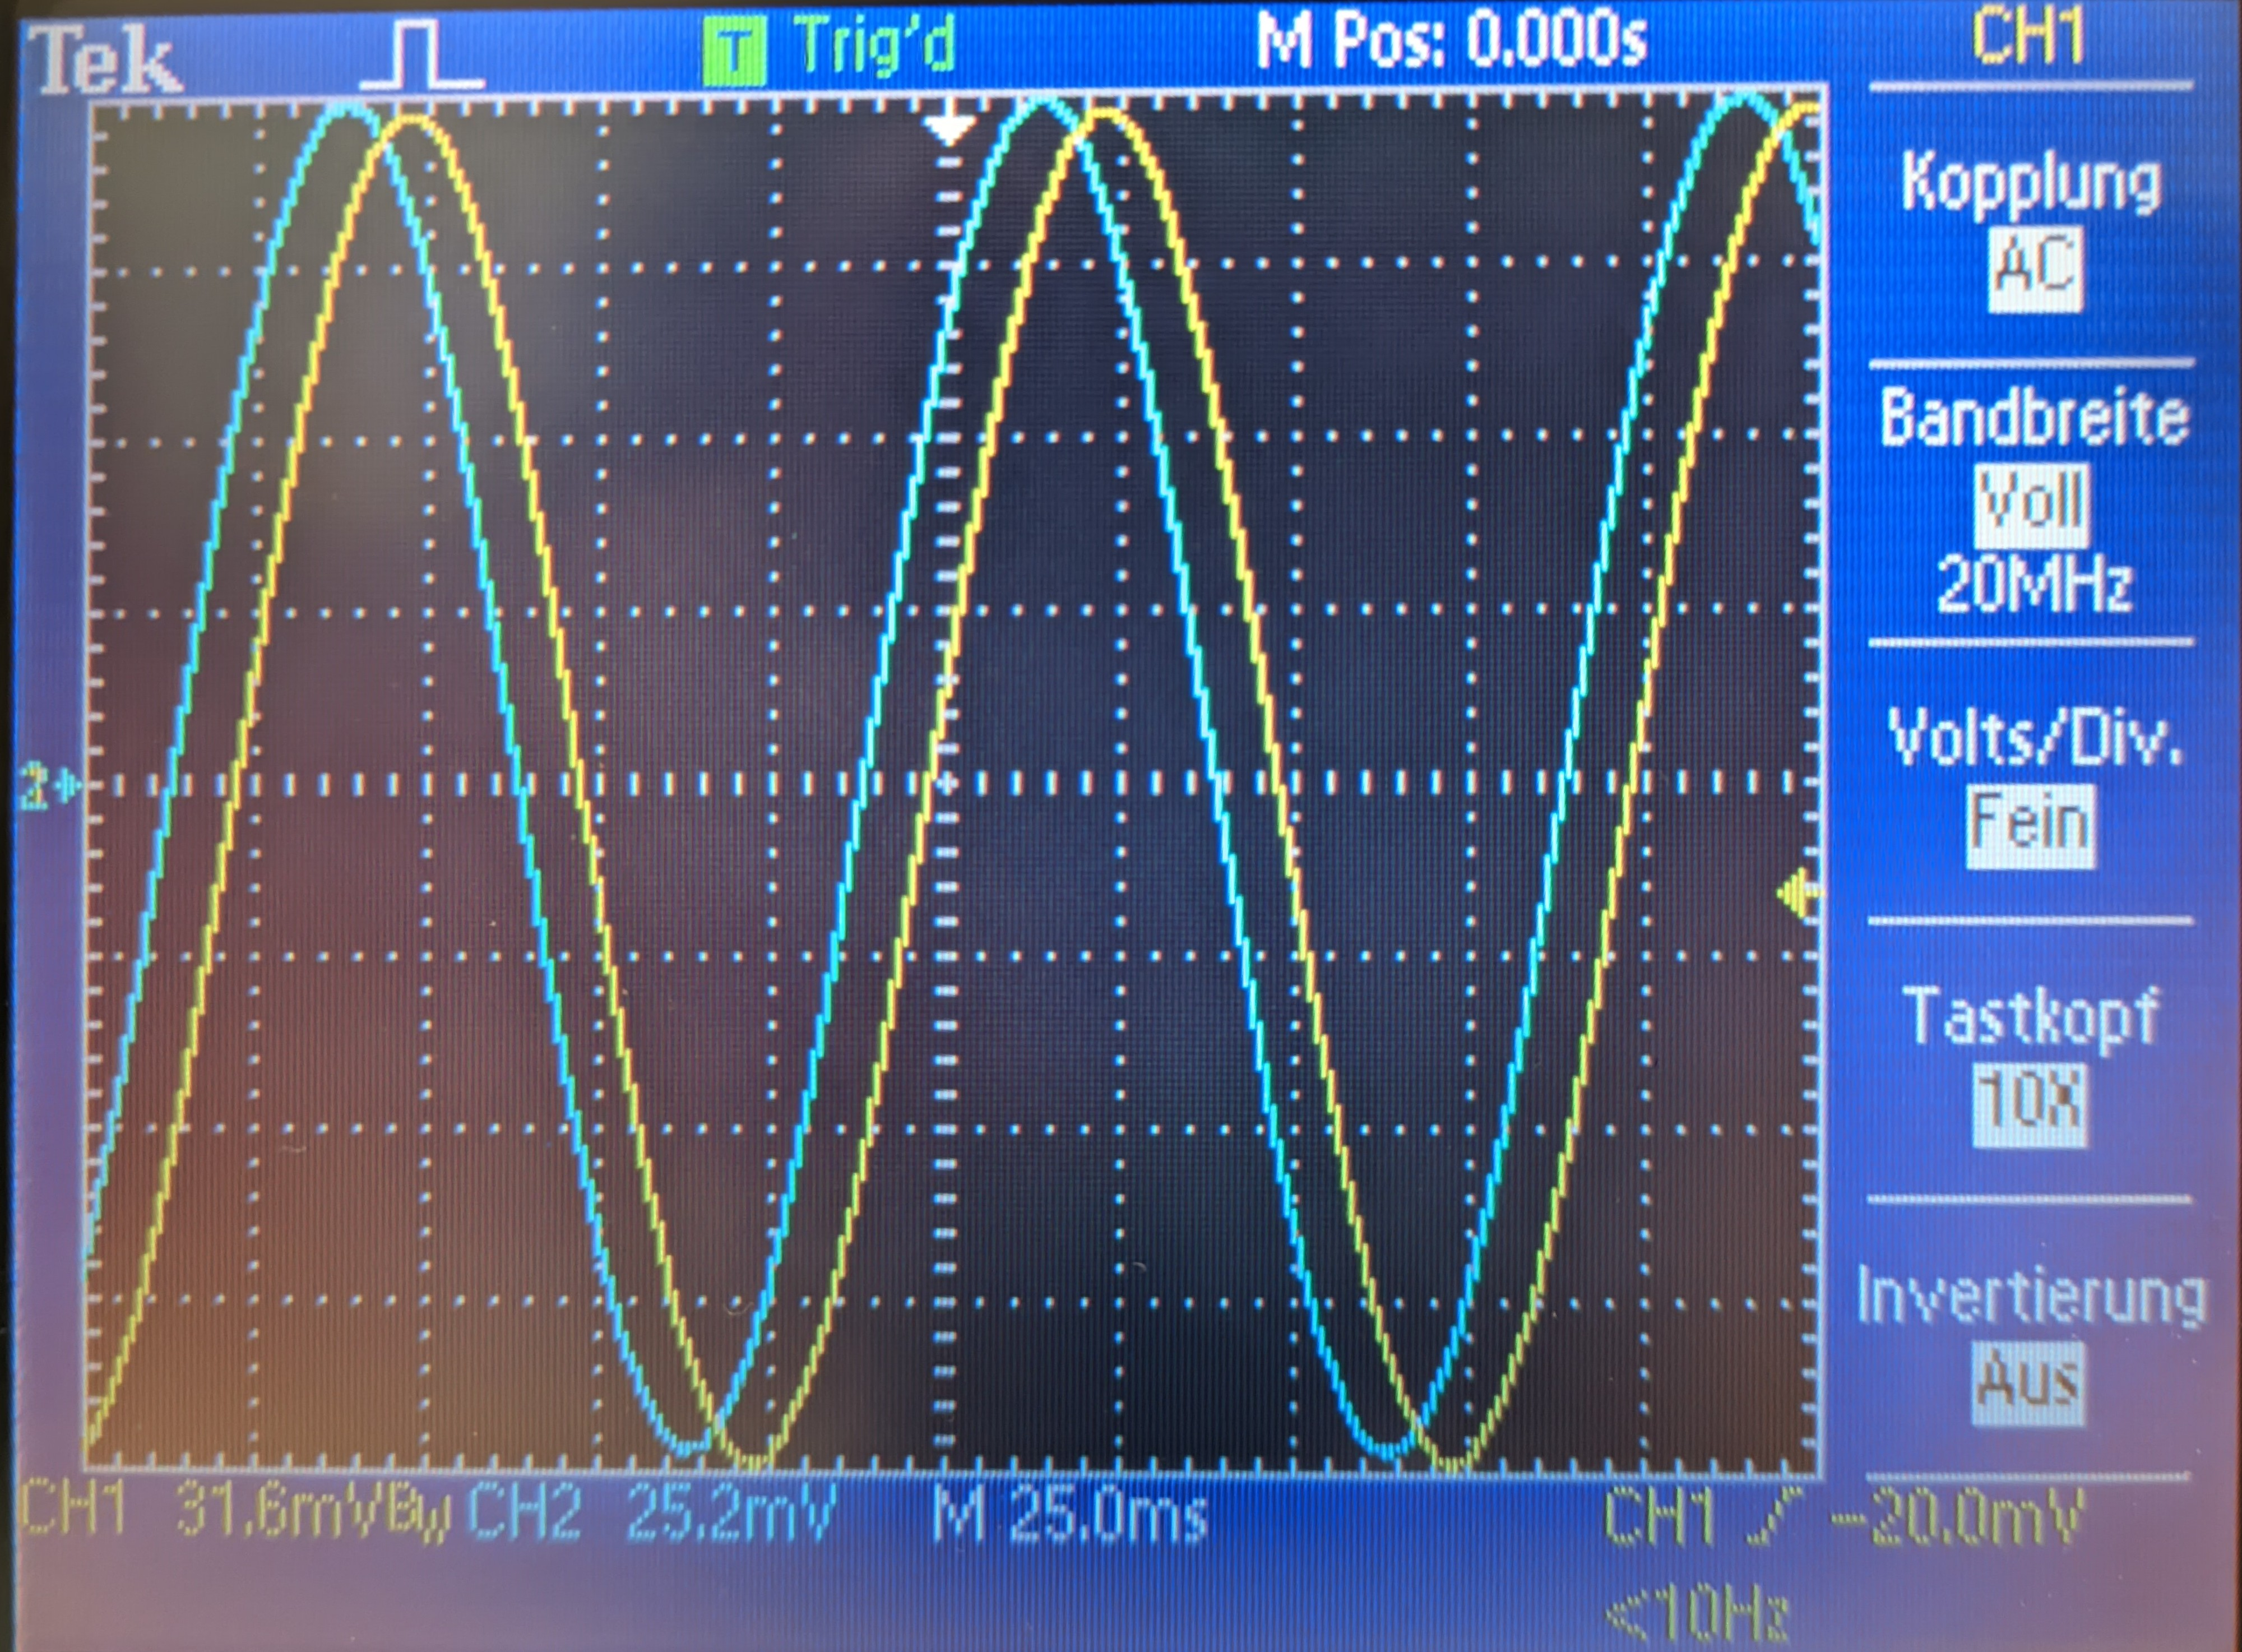
\includegraphics[width=0.95\textwidth]{./figures/integrator/sinussignal.jpg}
  \caption{Die Aufnahme vom Sinuseingangssignal(Gelb) und dem minus integrieten
  Ausgangssignal (Blau) bei einer Frequenz von \SI{10}{\hertz}. Die
  Einstellungen können dem Oszillogramm direkt entnommen werden.}
  \label{fig:mess_integrator_sinussignal}
\end{figure}

Nun wurde dasselbe mit einem Dreickseingangssignal
Sinuseingangssignal, siehe \autoref{fig:mess_integrator_dreiecksignal}, gemacht.

\begin{figure}[H]
  \centering
    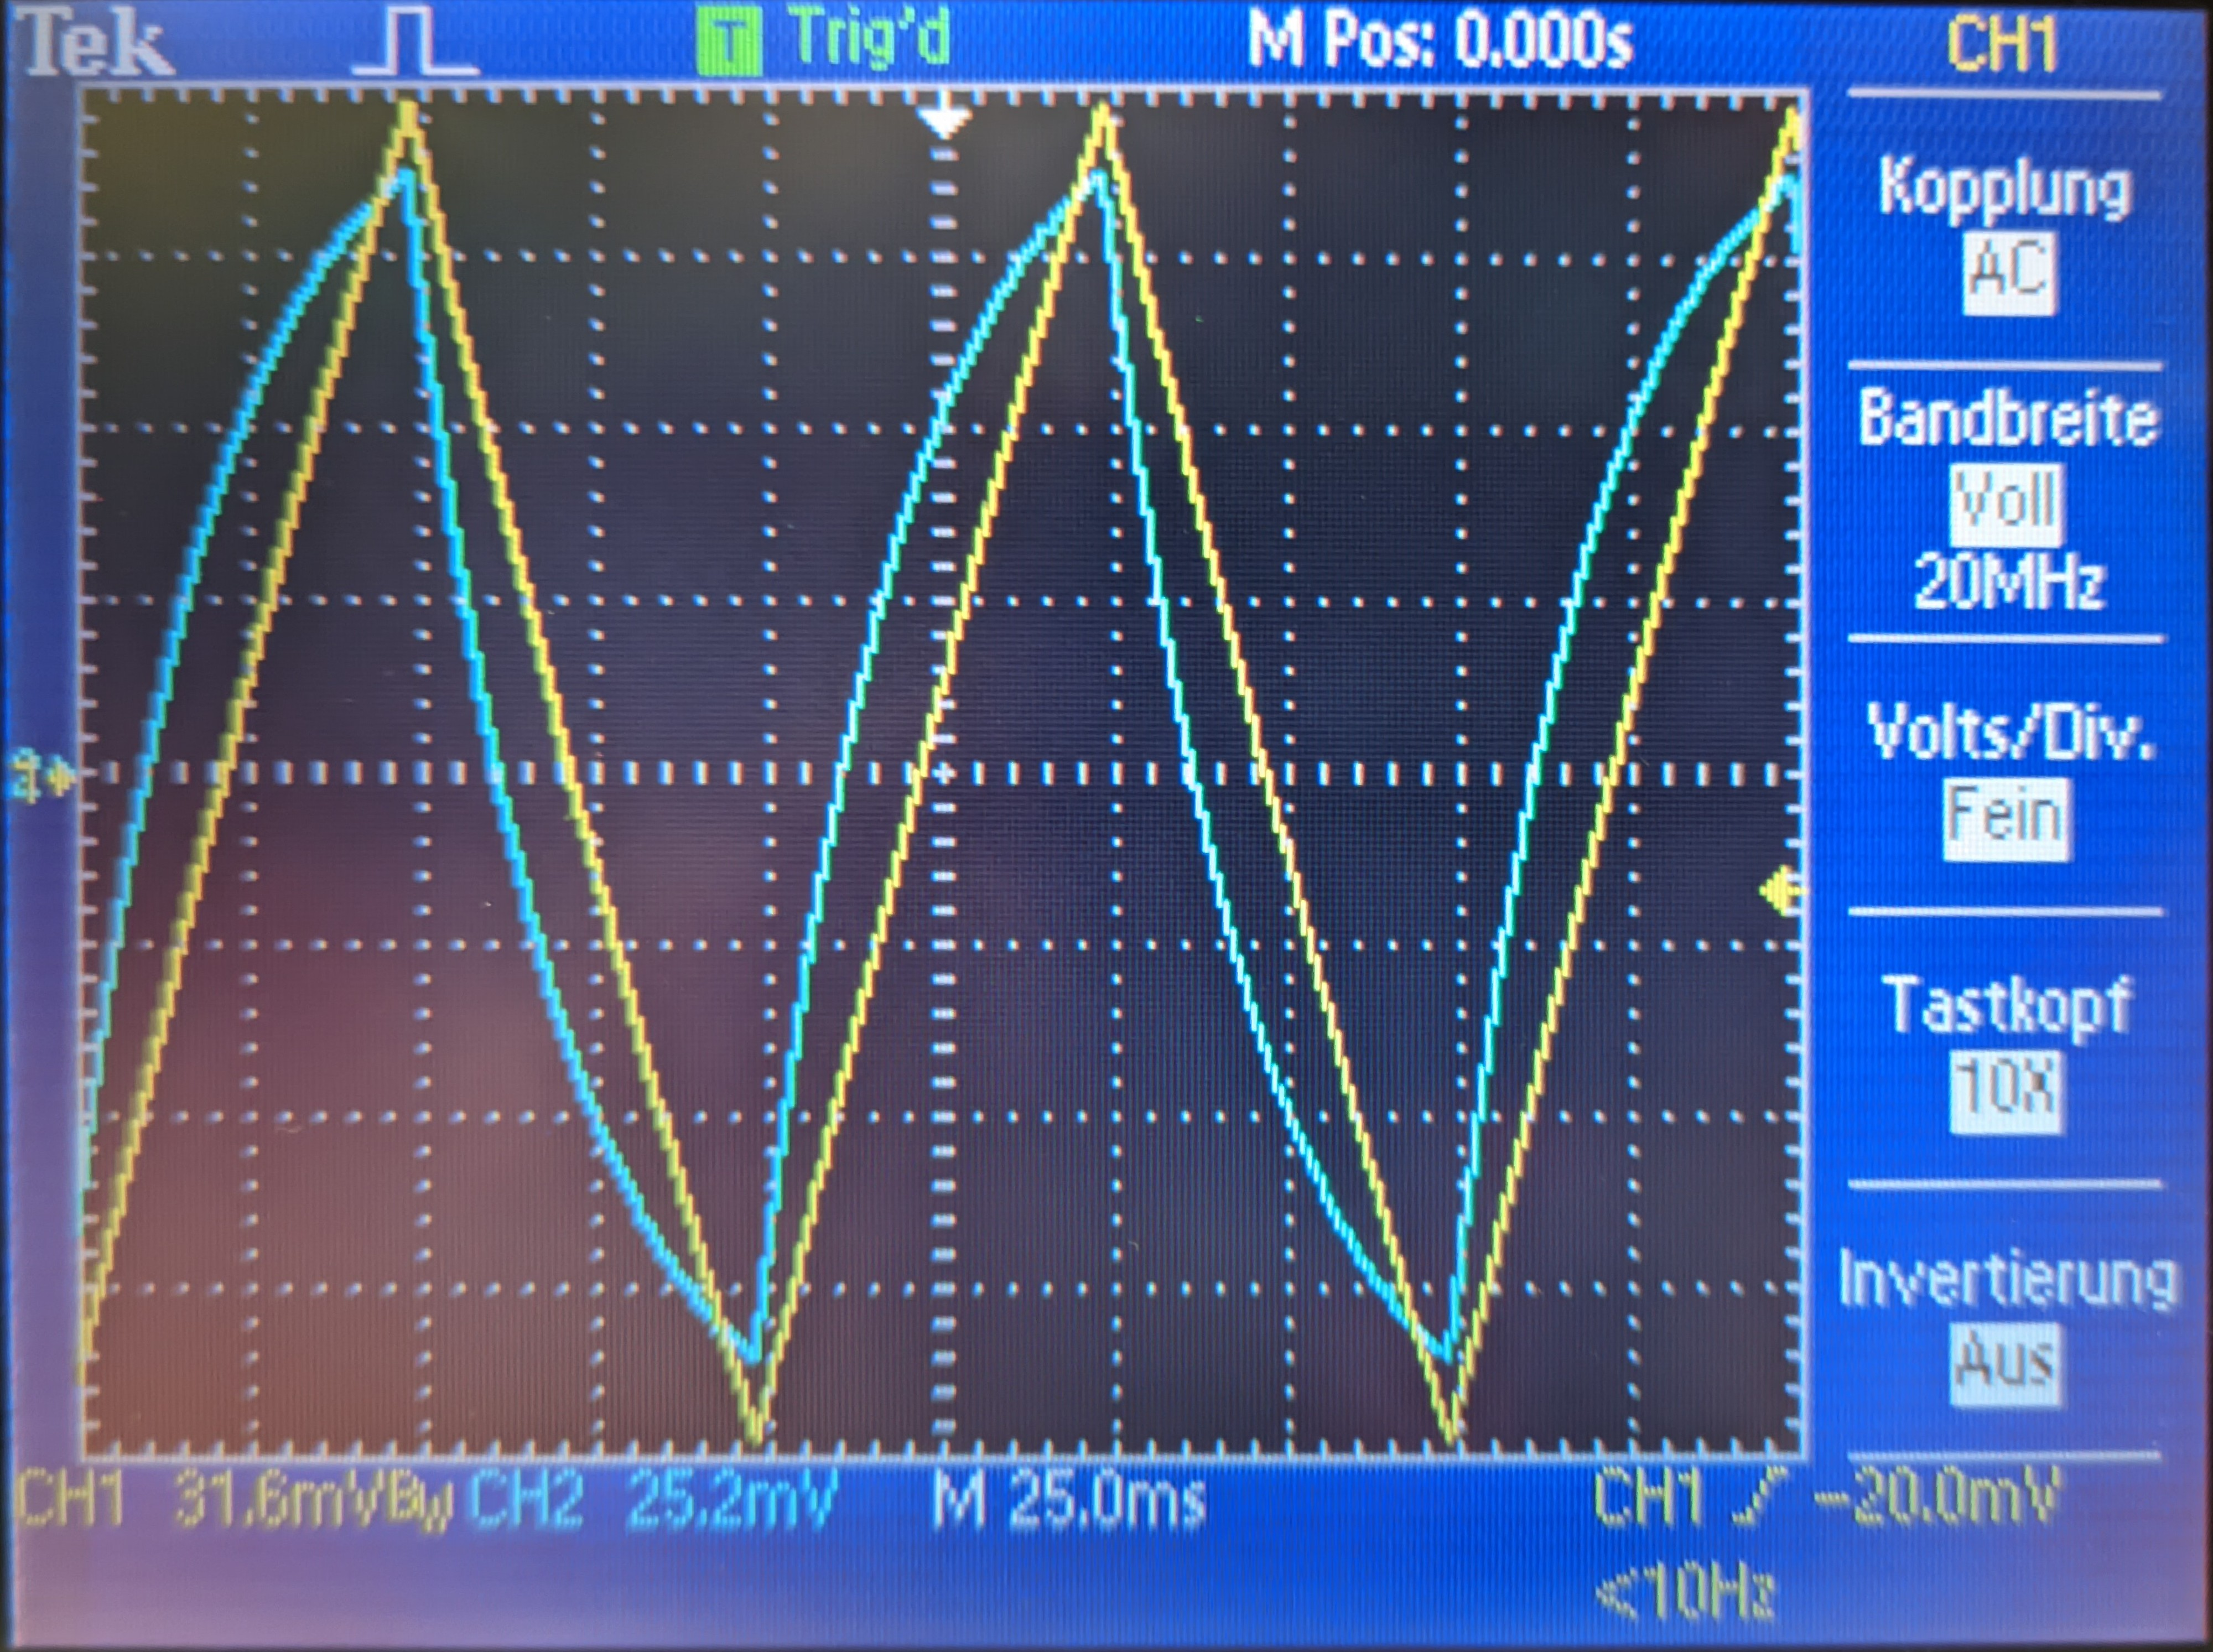
\includegraphics[width=0.95\textwidth]{./figures/integrator/dreiecksignal.jpg}
  \caption{Die Aufnahme vom Dreickseingangssignal(Gelb) und dem minus integrieten
  Ausgangssignal (Blau) bei einer Frequenz von \SI{10}{\hertz}. Die
  Einstellungen können dem Oszillogramm direkt entnommen werden.}
  \label{fig:mess_integrator_dreiecksignal}
\end{figure}

Da der Singalgenerator \cite{funktionsgenerator} keine Rechteckspannung erzeugen konnte, konnte
dies auch nicht mit einem Rechteckssignal untersucht werden.

% NOTE: Erwaehnen Rechteckspannung konnte nicht gemacht werden.

% 8) Vergleichen Sie die frequenzabhängige Verstärkung der Schaltung in einem Bereich
% zwischen 5 und 50 Hz mit der Simulation.
\paragraph{Untersuchung der frequenzabhänigen Verstärkung}
Zur Untersuchung der Frequenzabhängigkeit der Verstärkung des OPVs wurde wie im
Kapitel \nameref{sec:Aufgabenstellung} ersichtlich die Frequenz des
Sinuseingangssignals von \SIrange{5}{50}{\hertz} in 15er Schritten varriert.

\begin{figure}[H]
  \centering
    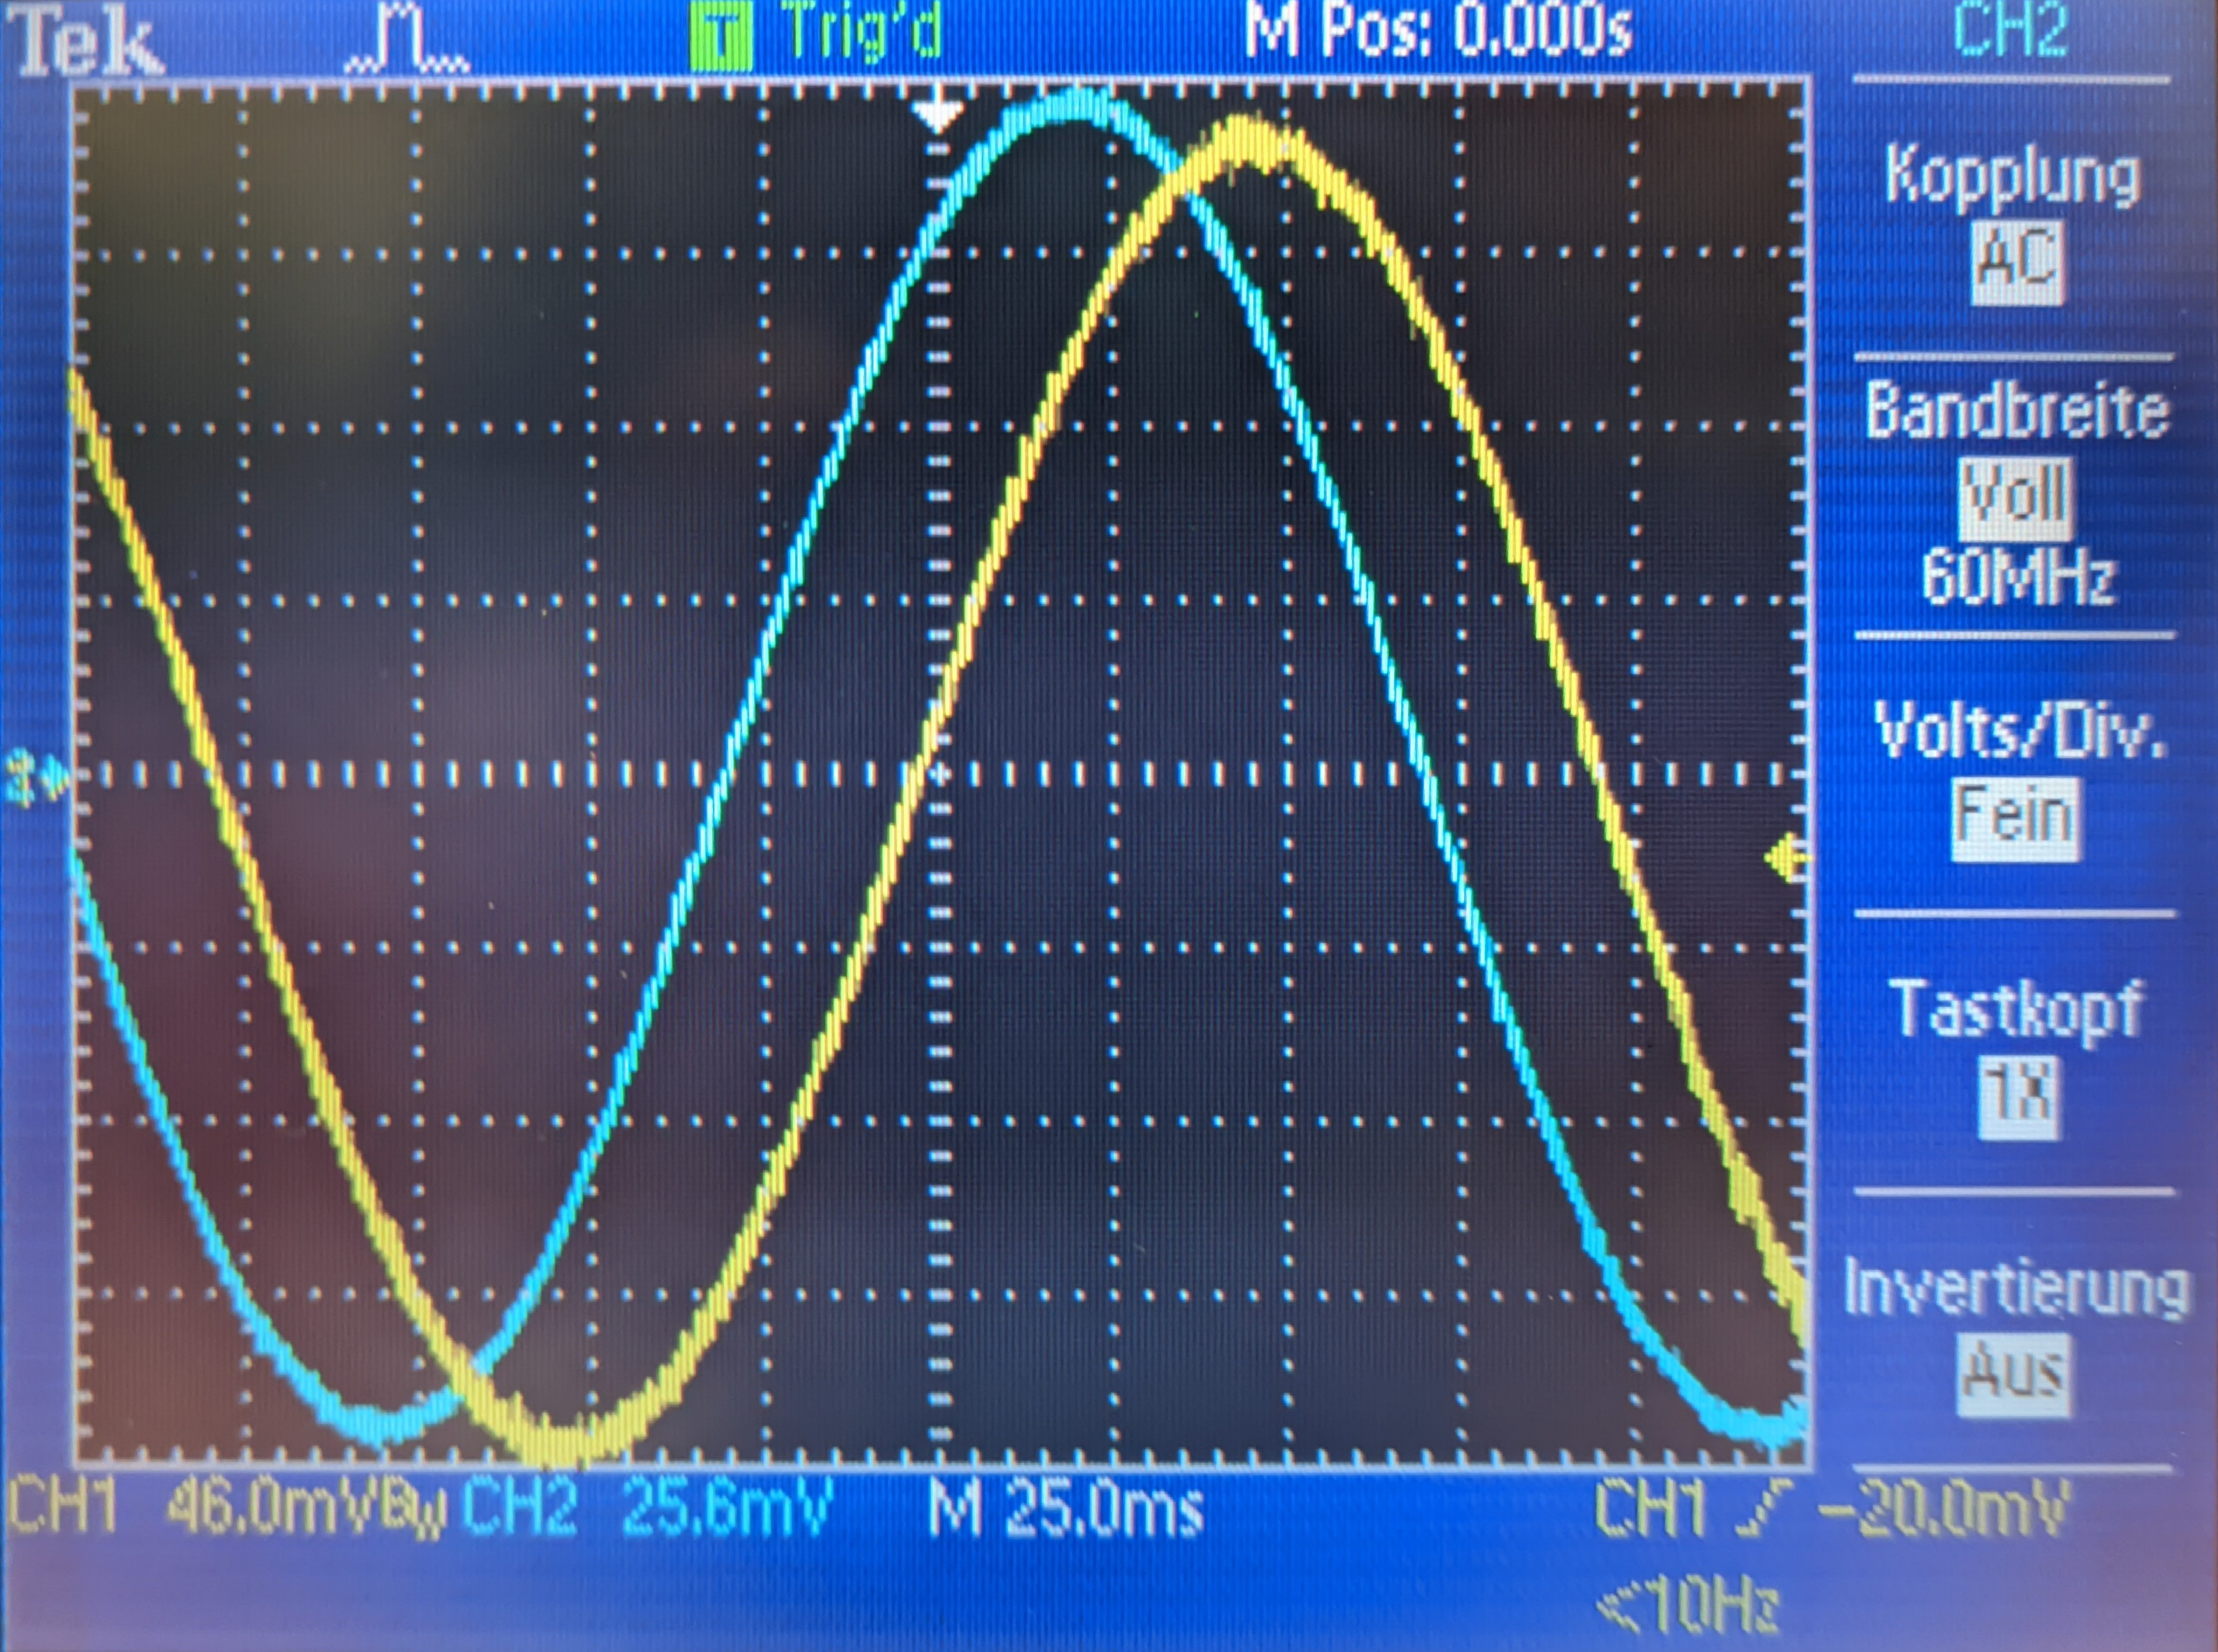
\includegraphics[width=0.95\textwidth]{./figures/integrator/5hz.jpg}
    \caption{In dieser Grafik ist das Sinuseingangssignal(Gelb) bei einer Frequenz von
    \SI{5}{\Hz} und dessen Ausgangssignal(Blau) ersichtlich.}
  \label{fig:mess_integrator_5hz}
\end{figure}

\begin{figure}[H]
  \centering
    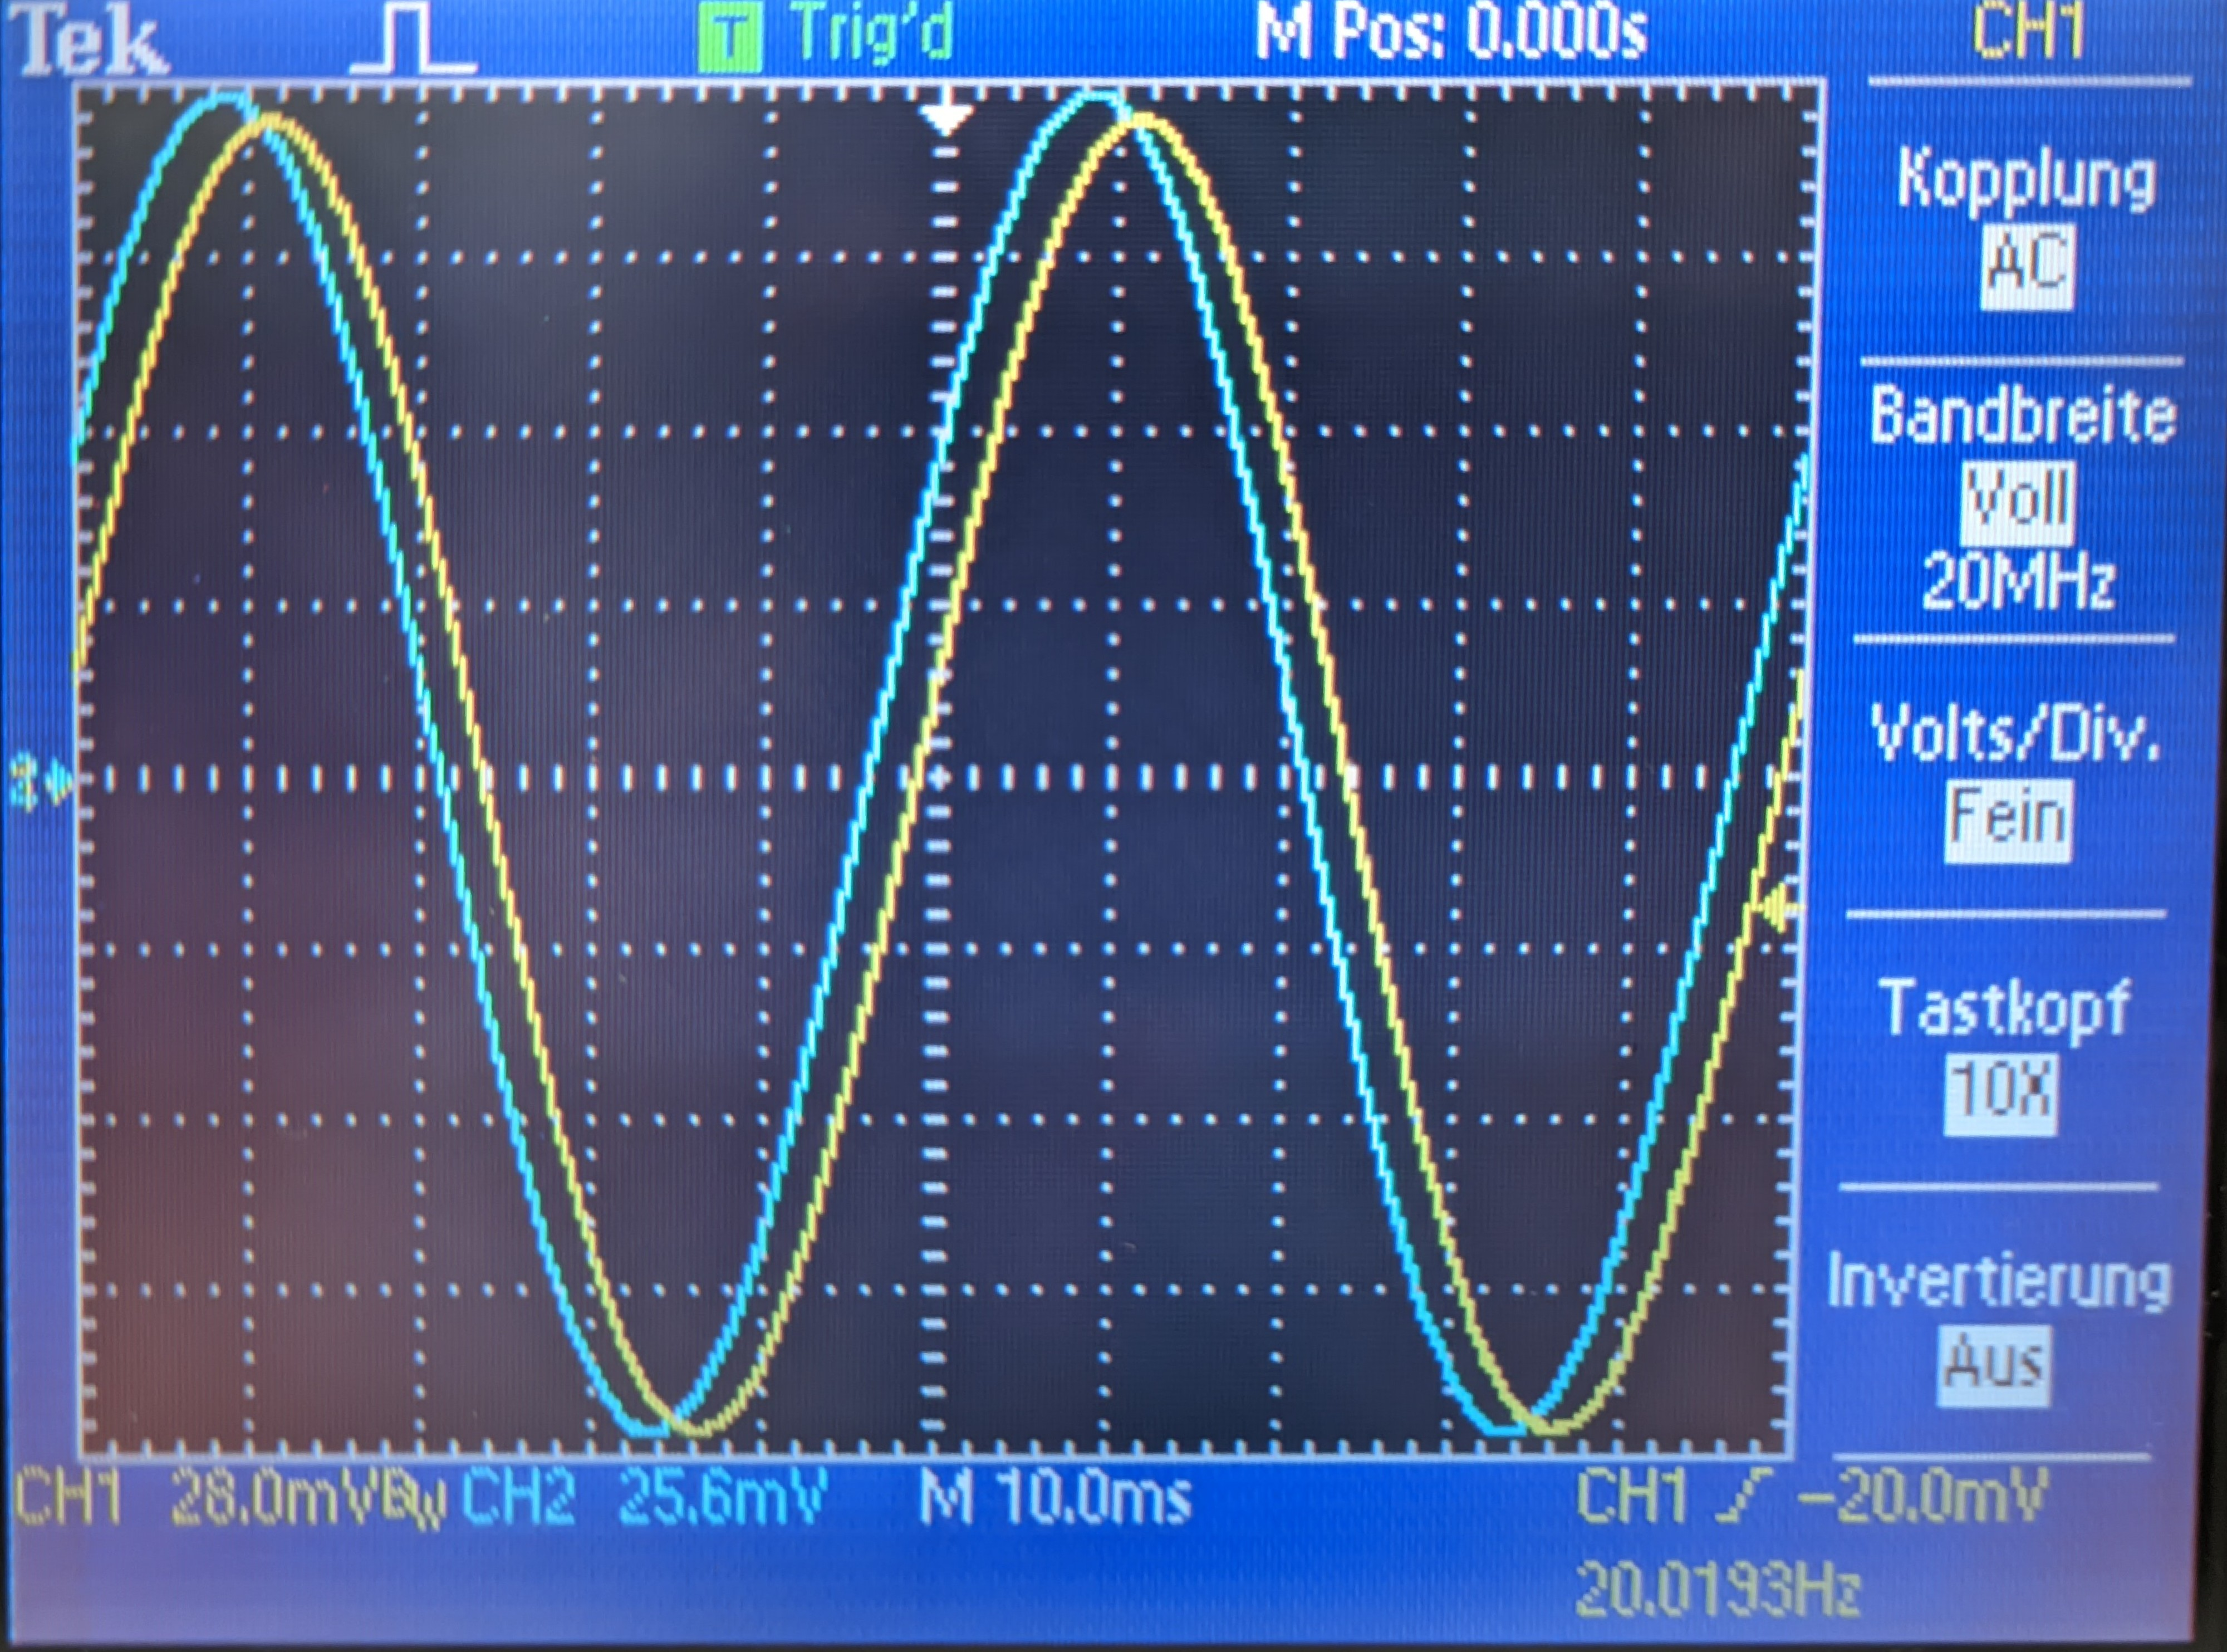
\includegraphics[width=0.95\textwidth]{./figures/integrator/20hz.jpg}
    \caption{In dieser Grafik ist das Sinuseingangssignal(Gelb) bei einer Frequenz von
    \SI{20}{\Hz} und dessen Ausgangssignal(Blau) ersichtlich.}
  \label{fig:mess_integrator_20hz}
\end{figure}

\begin{figure}[H]
  \centering
    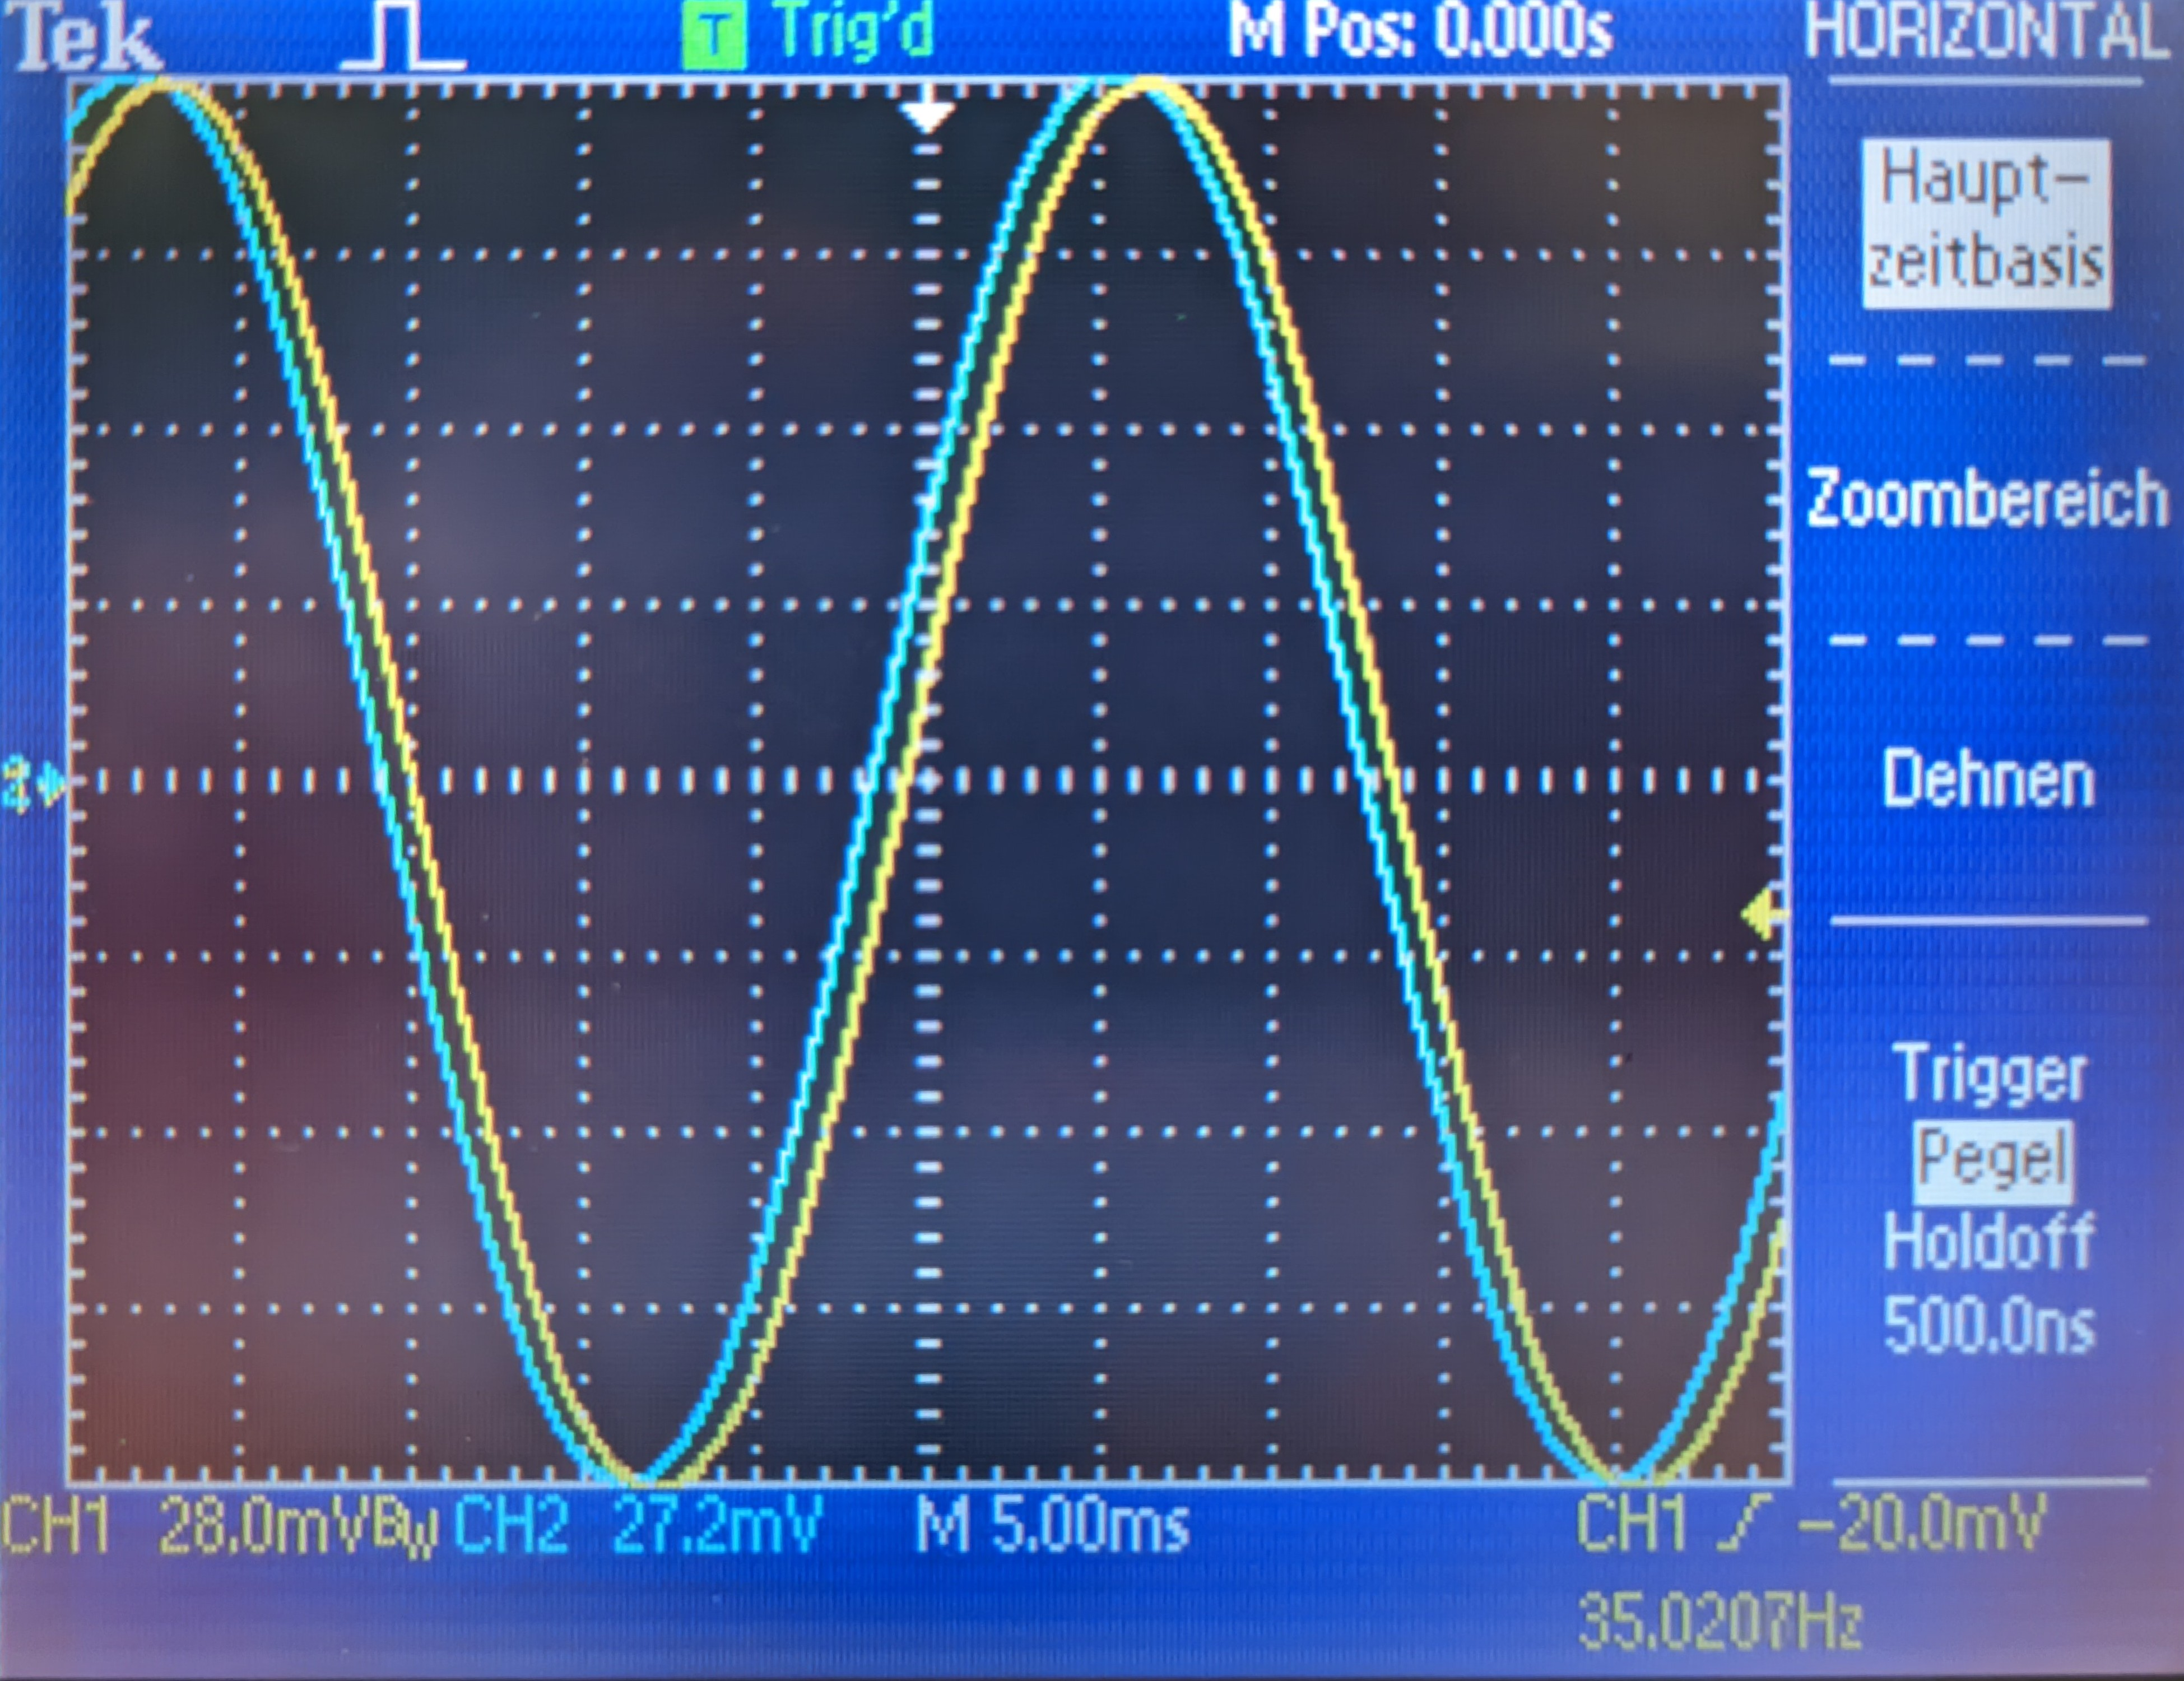
\includegraphics[width=0.95\textwidth]{./figures/integrator/35hz.jpg}
    \caption{In dieser Grafik ist das Sinuseingangssignal(Gelb) bei einer Frequenz von
    \SI{35}{\Hz} und dessen Ausgangssignal(Blau) ersichtlich.}
  \label{fig:mess_integrator_35hz}
\end{figure}

\begin{figure}[H]
  \centering
   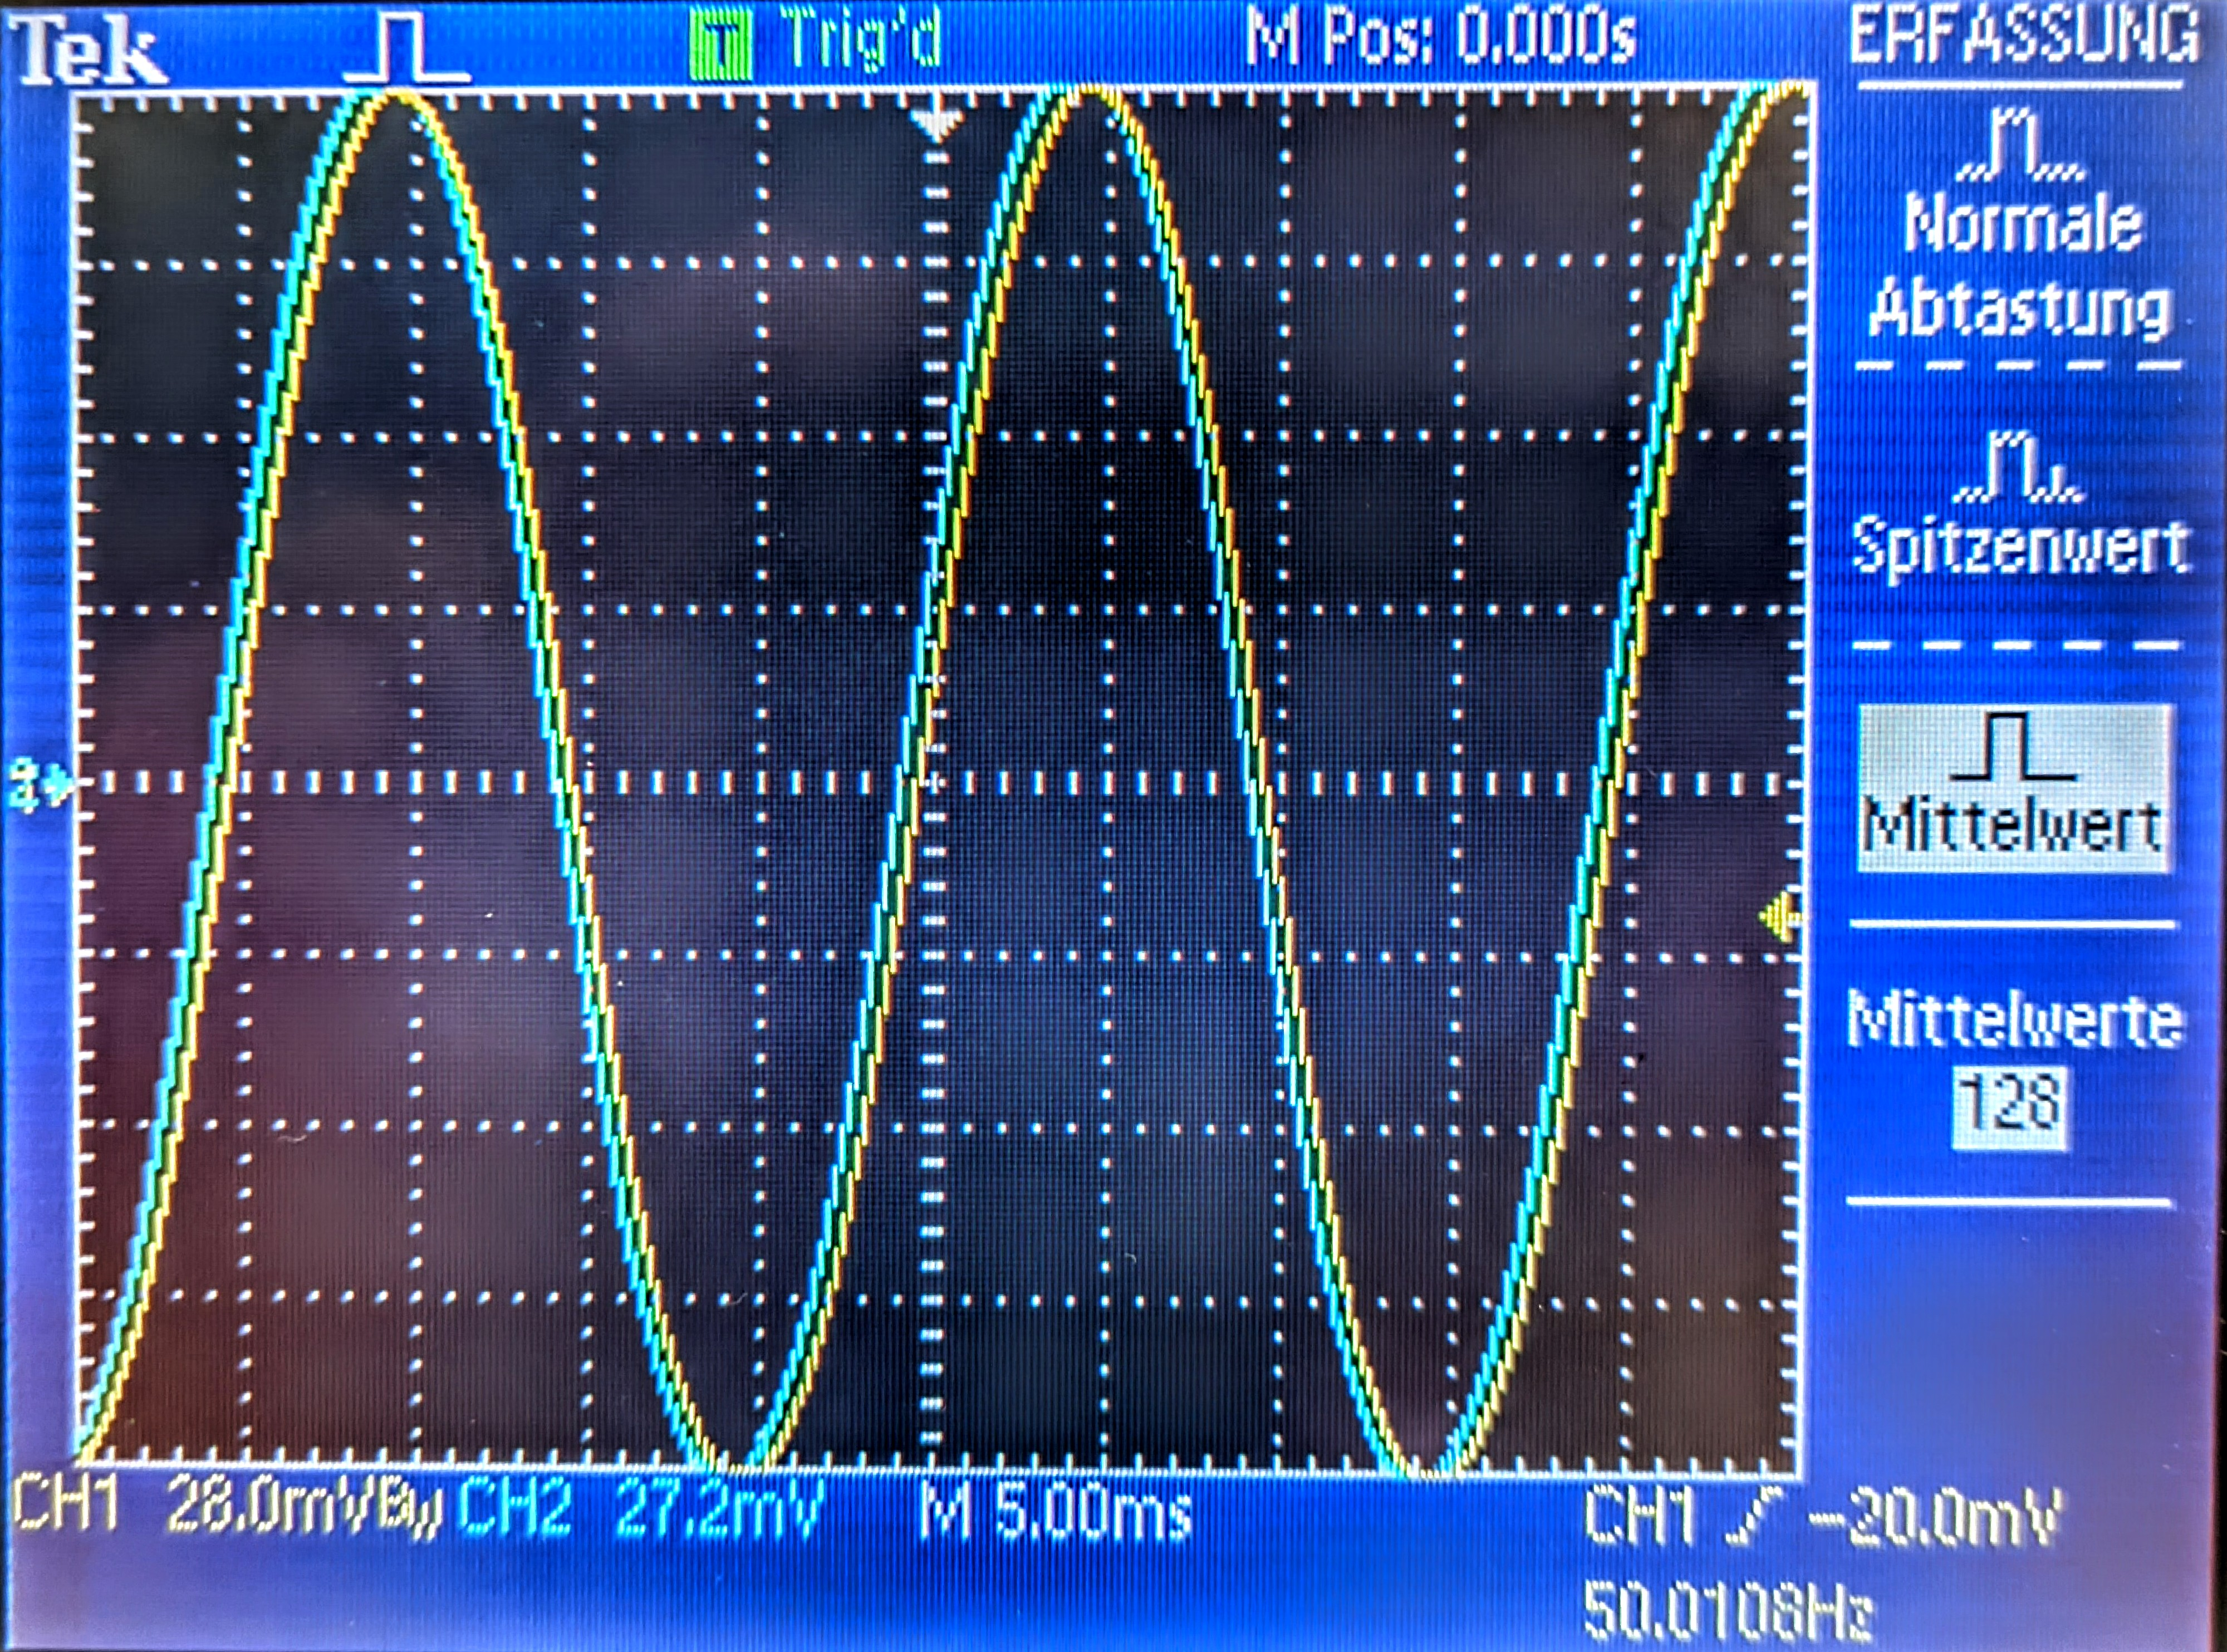
\includegraphics[width=0.95\textwidth]{./figures/integrator/50hz.jpg}
    \caption{In dieser Grafik ist das Sinuseingangssignal(Gelb) bei einer Frequenz von
    \SI{50}{\Hz} und dessen Ausgangssignal(Blau) ersichtlich.}
  \label{fig:mess_integrator_50hz}
\end{figure}

\paragraph{Simulation Untersuchung der frequenzabhängigen Verstärkung}

% 9) Die Simulation ist um die genannte Verstärkerstufe zu erweitern.
% Wiederholen Sie mit der neuen Schaltung Punkt 2 und 7
\subsubsection{Simulation des Integrators mit zusätzlicher Verstärkerstufe}

Schlussendlich wird die Integratorschaltung in der Simulation um eine
OPV-Verstärkerstufe gemäß \autoref{fig:sim_integrator_stufe_schaltung}
erweitert, wobei ein zweiter $\mu$A741 als Operationsverstärker in der
Verstärkerstufe verwendet wurde.

\begin{figure}[H]
  \centering
  % TODO LTSPICE aufbau der Elektrometer
    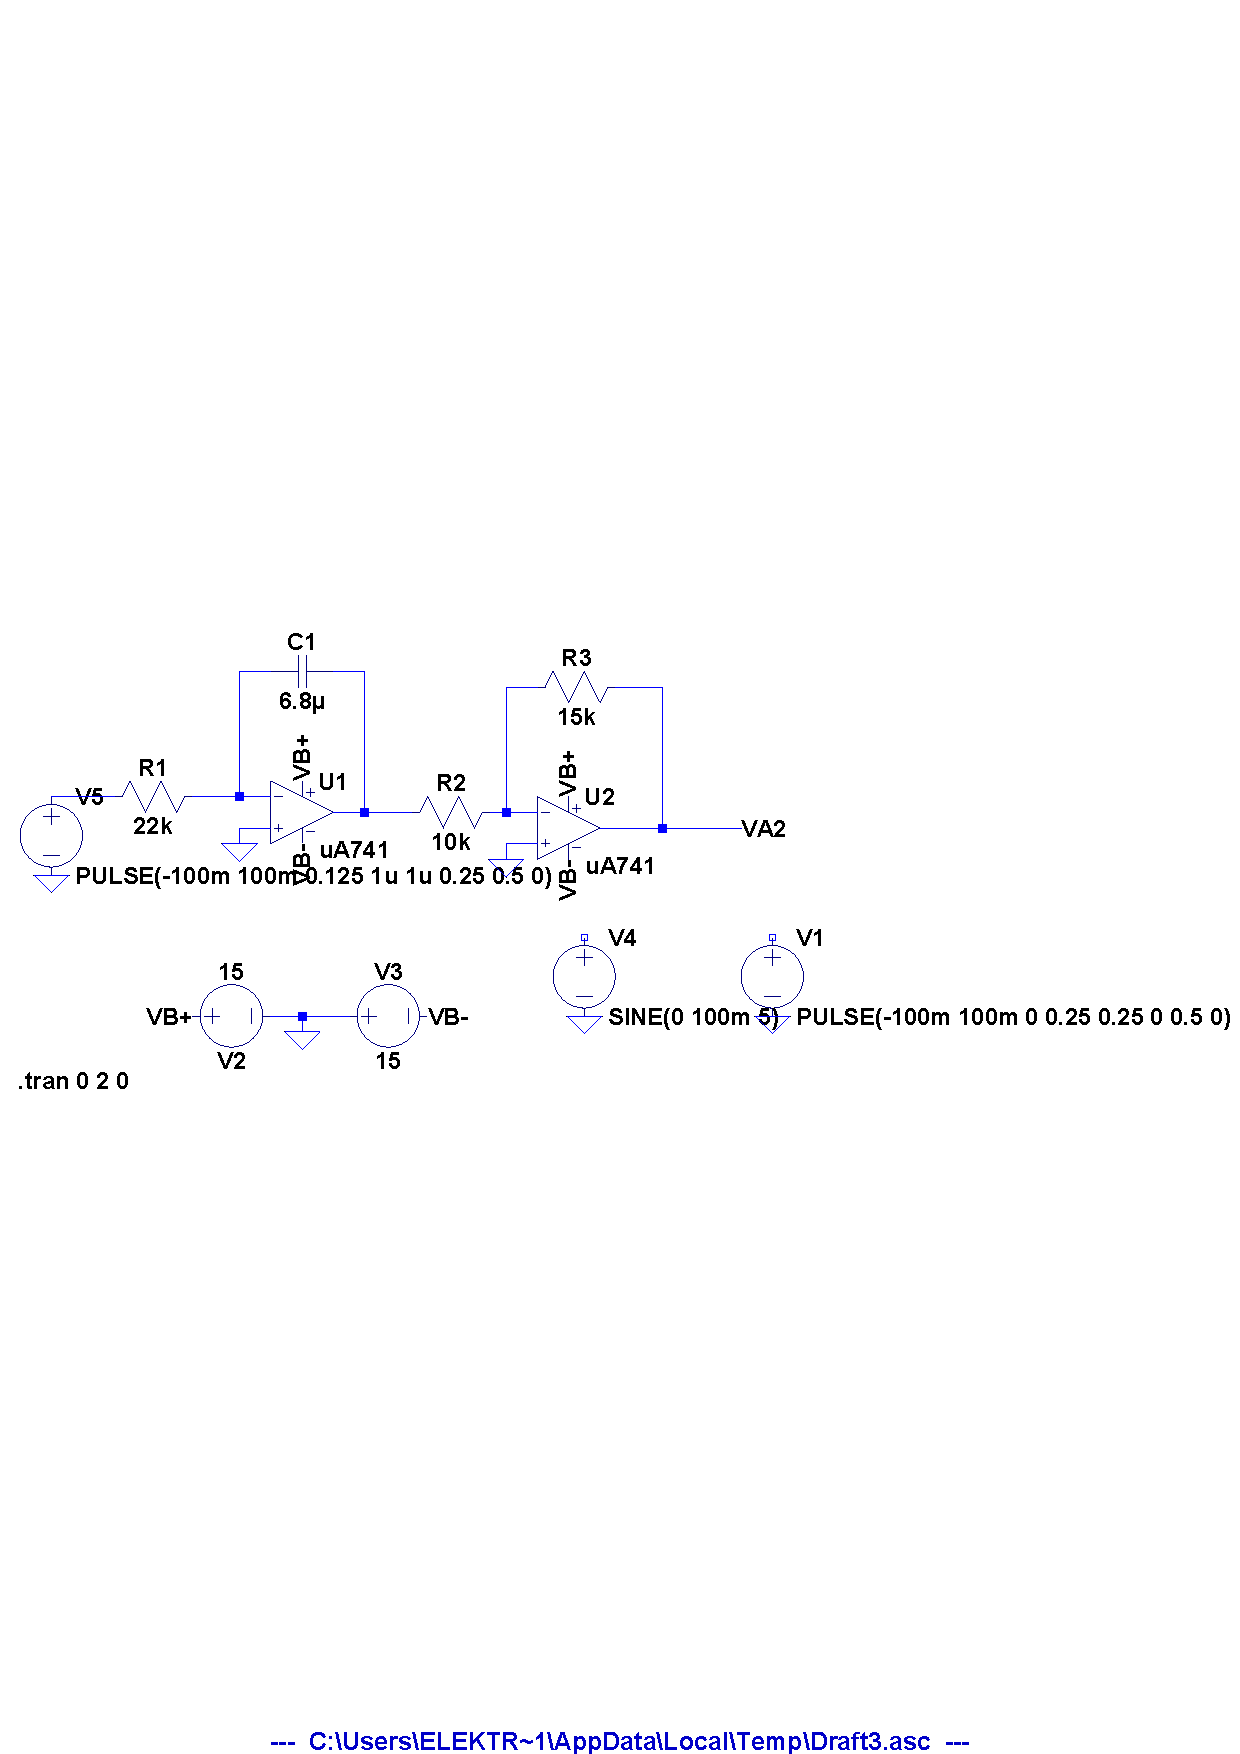
\includegraphics[width=0.95\textwidth]{./figures/integrator/sim/mit_stufe/schaltung_spannungstypen.pdf}
  \caption{Dies ist die Integratorschaltung mit Verstärkerstufe; aufgebaut in \textit{LTSPICE}.}
  \label{fig:sim_integrator_stufe_schaltung}
\end{figure}

Die Integrationszeit, nach welcher die Ausgangsspannung \SI{10}{\volt} beträgt,
wurde erneut graphisch mithilfe einer zeitliche Transienten-Analyse ermittelt,
wobei eine konstante Spannungsquelle von \SI{100}{\milli\volt} verwendet wurde.
Die Ausgangsspannung in Abhängigkeit der Zeit ist in
\autoref{fig:sim_integrator_stufe_integrationszeit} dargestellt.

\begin{figure}[H]
  \centering
  % TODO LTSPICE trans anal von lade vorgang 
    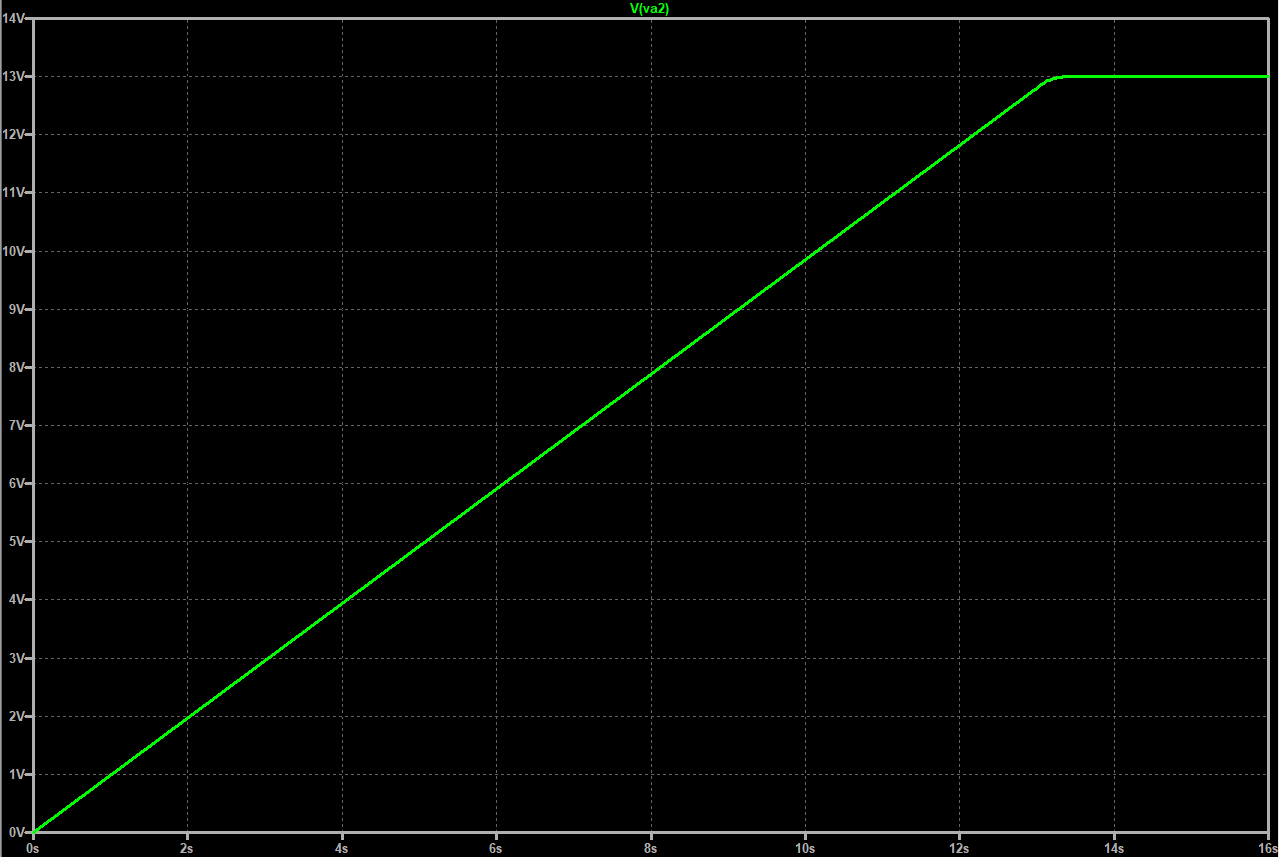
\includegraphics[width=0.95\textwidth]{./figures/integrator/sim/mit_stufe/100mv_aus_zeit.png}
  % TODO check spice directive, pathway
  \caption{Die Schaltung aus \autoref{fig:sim_integrator_schaltung} wurde auf
  die Integrationszeit untersucht, indem eine Transienten-Analyse vom
  Ladevorgang gemacht wurde. Die Simulation SPICE-Directive ist \texttt{.tran 0 16} 
  bei einer Eingangsspannung $U_e$ von \SI{100}{\milli\volt}.}
  \label{fig:sim_integrator_stufe_integrationszeit}
\end{figure}

Nun wurden wiederum verschiedene Spannungsquellen als Eingangssignal für den
Integrator mit Verstärkerstufe verwendet. In \autoref{fig:sim_int_stufe_sin}
sind die zeitlichen Verläufe der Eingangs- und Ausgangsspannung bei einem
Sinus-Eingangssignal mit einer Amplitude von \SI{100}{\milli\volt} und einer
Frequenz \SI{5}{\hertz} von ersichtlich. Analog sind Eingangsspannung und
Ausgangsspannung für eine Rechtecksspannung mit einer Amplitude von
\SI{100}{\volt} und einer Periodendauer von \SI{500}{\milli\second} in
\autoref{fig:sim_int_stufe_rect} dargestellt. In
\autoref{fig:sim_int_stufe_tri} sind die Verläufe von $U_e$ und $U_a$ für eine
Dreiecksspannung als Signalquelle zu sehen.
%todo: insert graphs sin, rect, tri

% zu 4: Auswertung siehe EPM Skript nur Besprechung von Umformungen und 
% Sachen die man mit den Messungen machen muss damit man Conclusion und Wissen 
% gewinnen kann.
% Entsprechend der in Punkt 2. angegebenen Beziehungen (Formeln) ist aus den
% Messergebnissen in Punkt 5. das in Punkt 1. formulierte Endergebnis zu
% berechnen. Oft ist eine Ermittlung des Endergebnisses aus einer grafischen
% Darstellung bzw. eine grafische Veranschaulichung zweckmaßig. Dabei kann
% die Verwendung von Millimeterpapier oder Computerprogrammen hilfreich sein.
% Wenn eine Bearbeitung der Daten auf dem Computer erfolgt, sollte bei der
% Darstellung der Graphen eine sinnvolle Skalenteilung des Koordinatensystems
% gemacht werden. Die Unsicherheitsbetrachtung f ̈ur die angegebenen Messwerte,
% sowie fur Zwischen- und Endergebnisse ist in diesem Abschnitt
% nachvollziehbar zu beschreiben. Dabei ist nach Kapitel 1 vorzugehen und
% insbesondere auf die Klassifizierung der Unsicherheit (Typ-A/B) und die
% Unsicherheitsfortpflanzung einzugehen.
\section{Auswertung}\label{sec:Auswertung}

\subsection{Simulation}

\subsection{Steckbrett}

\subsubsection{Verstärkung \& Aussteuerungsbereich}
Damit die Verstärkung in des Elektrometerverstärkers bestimmt werden kann wurde
der lineare Bereich in den Daten aus \autoref{tab:mess_elektro_aussteurerung}
gefittet. Da die Steigung der Vertärkung entspricht zu finden.
\subsubsection{Integrationszeit}
Die Integrationszeiten aus \autoref{tab:messungen_integration} wurden gemittelt
und die Messung wurde als Gaußverteilt stattgefunden.

% zu 5: Diskussion und Zusammenfassung
% In der Zusammenfassung stehen noch einmal die wichtigsten Messergebnisse, wobei auf Tabellen und
% Abbildungen nur verwiesen werden soll. Die Ergebnisse sind auch zu diskutieren. Insbesondere müssen
% Abweichungen zwischen Simulation und praktischer Durchführung diskutiert werden.
\section{Diskussion und Zusammenfassung}\label{sec:Diskussion} 
\subsection{Diskussion}
\subsubsection{Elektrometerverstärker}
\paragraph{Aussteuerung}
%ausstereung: 0,6-0,9x der Ub sollte Ua bei Aussteuerung max sein -> sättigung
Die Aussteuerung eines Operationsverstärkers soll bei einer Ausgangsspannung
des 0,6 bis 0,9-fachen der Betriebsspannung erreicht werden, was bei einer
Betriebsspannung von \SI{\pm 15}{\volt} eine Spannweite von \SI{\pm 9}{\volt}
bis \SI{\pm 13,5}{\volt} ergibt. Wie in \autoref{fig:sim_elektrometer_dcsweep}
für den Elektrometerverstärker zu sehen, deckt sich dieser Verhalt mit der
Simulation, bei welcher die Aussteuerung ab einer Eingangsspannung von \SI{\pm
200}{\milli\volt} auftritt, wobei eine maximale Ausgangsspannung von \SI{\pm
13}{\volt} erreicht wird. Der Verlauf ähnelt dabei stark der charakteristischen
Kennlinie der Ausgangsspannung eines gewöhnlichen OPVs. Die Sättigungen im
Aussteuerungsbereich, die ebenso bei einer Ausgangsspannung von \SI{\pm
13}{\volt} erreicht werden, sind auch anhand der Simulationen der
Integrationszeit der Integratorschaltung in
\autoref{fig:sim_integrator_integrationszeit} für die Schaltung ohne respektive
in \autoref{fig:sim_integrator_stufe_integrationszeit} für die Schaltung mit
Verstärkerstufe deutlich zu erkennen. 

Die Messung der Ausgangsspannung unter Variation der Eingangsspannung am
Steckbrett ergibt, wie in \autoref{fig:} zu sehen, 
einen qualitativ sehr ähnlichen Verlauf der Datenpunkte. 
%todo: insert fig name for scatter plot
Dabei tritt die Sättigung ab einer Eingangsspannung von etwa \SI{\pm 220}{\volt} 
auf, wobei die maximale Ausgangsspannung auf der positiven Achse
ca. \SI{13,9}{\volt} und auf der negativen \SI{-13,5}{\volt} beträgt. Diese
geringfügigen Abweichungen von der Simulation sind wohl auf das reale Verhalten
der Schaltung (u.a. Temperaturabhängigkeit der Bauelemente) zurückzuführen und
so zu erwarten gewesen.

\paragraph{Ausgangsspannung Steckbrett}
Ziel der Elektrometerverstärker-Schaltung war eine Eingangsspannung von
\SI{125}{\milli\volt} in eine Ausgangsspannung von \SI{8}{\volt} umzuwandeln.
Dies wurde am Steckbrett gemäß \autoref{eq:messwert_elektro_ausgang_eingang}
mit ähnlich hoher Genauigkeit wie bei der Simulation erzielt. Die Abweichung
beträgt demzufolge nur \SI{30}{\milli\volt}, was bei einer Größenordnung von
mehreren Volt vernachlässigbar ist und eine ausreichende Genauigkeit
gewährleistet.

\subsubsection{Integrator}
\paragraph{Integrationszeit}
Die in der Simulation für den Integrator ohne Verstärkerstufe bestimmte
Integrationsdauer von \SI{15,1}{\second} (siehe
\autoref{fig:sim_integrator_integrationszeit}), die verging bis eine anvisierte
Ausgangsspannung von \SI{-10}{\volt} erreicht wurde, weicht kaum von den Werten
der Vorbereitung (siehe \autoref{sec:Vorbereitung}) ab. Dabei sollte für die
gegebene konstante Spannungsquelle von \SI{100}{\milli\volt} die
Integrationszeit \SI{15}{\second} betragen. Im Rahmen des Versuchs an der
Steckplatine ergab sich bei sechsmaliger Durchführung ein Wert von
\SI{}{\second}.
% TODO discuss the discreptency in the time measurement with the expected result 
%todo: insert int time 

Für die Integratorschaltung mit Verstärkerstufe sollte gemäß der Vorbereitung
in \autoref{sec:Vorbereitung} bei einer Eingangsspannung von
\SI{100}{\milli\volt} nach \SI{10}{\second} eine Ausgangsspannung von
\SI{10}{\volt} erreicht werden. Mittels der Simulation wurde die
Integrationszeit zu \SI{10,1}{\second} aus
\autoref{fig:sim_integrator_stufe_integrationszeit} bestimmt. Abgesehen von der
erneut nur marginalen Abweichung von \SI{0,1}{\second}, die wohl auf die
Näherungen der Widerstände zurückzuführen ist, impliziert dies, dass die
Schaltung wie geplant funktioniert und erfolgreich konstruiert respektive
dimensioniert wurde.

\paragraph{Spannungsarten}
Die Eingangs- und Ausgangsspannungen sind in \autoref{} 

%frequenzabhängigkeit: opv-schaltung mit rückkopplung; größere variation wäre gut -> bode
%integrationszeit: nahe zielwert, gute Dimensionierung



% TODO discuss the discreptency in the time measurement with the expected result 

%Es wäre wohl vernünftiger gewesen, die Schaltung an der Steckplatine zunächst aufzubauen, um etwaige 
%Ungenauigkeiten durch die Widerstände 
\subsection{Zusammenfassung}

\newpage

\printbibliography

\listoffigures

\listoftables



\end{document}
